
%
%%%%%%%%%%%%%%%%%%%
%                 %
% Energy Models   %
%                 %
%%%%%%%%%%%%%%%%%%%
%
% Brief abstract: contains the energy models that are later employed for replanning and scheduling
%
% Completion (1-10): 9
% Missing: some explanations on aperiodic models, summary, results, two figures
%
\chapter{Energy Models}
\label{cp:model}

\begin{chapquote}{\cite{ondruska2015scheduled}}
  ``Robots require energy to operate. Yet they only have access to limited energy storage during missions.''
\end{chapquote}

\vspace*{1em}

\lettrine{E}{nergy is an essential aspect} of many autonomous mobile robotics scenarios~\citep{mei2005case} and often a limiting factor to improving computing performance~\citep{horowitz2014computing}. In the previous chapters, we emphasized the growing importance of both computations and motion energy components. Indeed, limited energy availability against high computing performance requirements of autonomous aerial robots is the motivation for the energy-aware coverage planning and scheduling for autonomous aerial robots in this work. For this purpose, we first need an accurate energy model that predicts future energy consumption. We derive such a model in this chapter, providing different energy models predicting the energy of the motion and computations and the battery state of an aerial robot. For the former two, we first derive a way to accurately predict the energy spent running a given set of computations on the computing hardware. We then merge the resulting computations energy model with a motion energy model using some properties of our autonomous scenario.  The energy output of the motion model is the input of the battery model, which predicts the battery evolution over time.

We saw in \fref{cp:model}{Chapter} some computations energy and battery models, and we discussed some energy-aware approaches for aerial robots (and mobile robots broadly) performing coverage path planning (\Gls{acr:cpp}) or motion planning generally. In this chapter, we then use the previous literature and derive the energy models for our scenario: an autonomous aerial robot employed in coverage planning, monitoring an agricultural field. Although applied to a given use case, the approach is general in terms of the proposed methodology. In \fref{sec:comp-ener-model}{Section}, we derive the model for the energy of computations based on regressional modeling. In \fref{sec:battery-model}{Section}, we provide a battery model based on an equivalent electrical circuit, and in \fref{sec:periodic-model}{Section}, we derive a model for the motion that incorporates the computations energy model. We then use the models in \fref{cp:dyn}{Chapter} to plan and schedule altogether.

This chapter connects to the remainder of this work as follows. We provided some energy implications of autonomous aerial robots in \fref{cp:intro}{Chapter} and formulated the basic constructs in \fref{cp:pb}{Chapter}, including the concepts of computations and motion energy. We discussed the past energy modeling and efficiency studies in \fref{cp:soa}{Chapter}, along with other literature. We then use all the information we discussed in the previous chapters for the energy models in this chapter. In \fref{cp:dyn}{Chapter}, we use the models to replan the coverage and schedule the computations in an energy-aware fashion. The replanning uses some optimal control techniques that we introduce in \fref{cp:opt}{Chapter}.


%%%%%%%%%%%%%%%%%%%%%%%%%%%%%%%%%%%%%%%%%%
\section{Energy Model of the Computations}
\label{sec:comp-ener-model}

This section describes the computations energy model to predict the energy consumption of a given configuration of computations. In \fref{sec:definitions}{Section} and the precision agriculture example in \fref{sec:computation-wise}{Section}, we parametrized the computations by a set of $\sigma$ computations parameters $c_{i}^\sigma:=\{c_{i,\rho+1},\dots,c_{i,\rho+\sigma}\}$, where $\rho$ is the number of path parameters. We parametrize the computations that impact the overall energy consumption (as we described in \fref{def:comps}{Definition}). For instance, in the agricultural scenario, we parametrize the computation object detection. We mean by parametrization that we enable the computations to be dynamically replanned with an appropriate choice of the parameters, and run on, e.g., a lower/higher rate requiring lower/higher power. Practically, this means that if our system is composed of $\sigma$ computations, the configuration of computations parameters $c_i^\sigma(\mathcal{T})$ for each stage $i$ over time $\mathcal{T}:=[t_0,t_l]$ (where $t_0,t_l$ are respectively the first time instant and the time instant when the aerial robot reaches the final point $\mathbf{p}_{\Gamma_l}$ in \fref{def:trigs}{Definition}) is a schedule of the computations. In \fref{cp:dyn}{Chapter}, we will derive an energy-aware schedule via the model that we propose in this section.
In the remainder of this section, we derive an energy model that maps any choice of parameters $c_{i}^{\sigma}$ to the power at any $t\in\mathcal{T}$, extending the past work on energy modeling for heterogeneous computing hardware.

In \fref{sec:model-hete-elem}{Section}, we summarize the heterogeneous elements modeling from \fref{sec:soa-ene-hete}{Section} and outline our approach, which consists of two layers. We detail the layers in \fref{sec:measurement-layer}{Sections}\fref{sec:predictive-layer}{--\hspace{-.8ex}} and describe an automated modeling tool we developed in \fref{sec:powprof}{Section} along with its configuration specification in \fref{sec:conf-spec}{Section}. The tool works well for computing hardware equipped with internal power meters, yet, some computing hardware does not provide any. We discuss how to model such hardware also in \fref{sec:powprof}{Section}.


\subsection{Model for the heterogeneous elements}
\label{sec:model-hete-elem}

We saw in \fref{cp:pb}{Chapter} that traditionally, models for computing hardware focus on a specific computing element, such as CPU or GPU, or model the elements heterogeneously. The models provide a regression function (measuring the power consumption over time), analytical (using some architectural parameters), or other expressions to infer future energy consumption. The regression functions, analytical or other expressions might depend on low-level architectural parameters and be employed in an energy-efficient selection of such parameters, including voltage and frequency. Alternatively, they might depend on high-level parameters (such as the computations parameters $c_{i}^\sigma$ in this work) and be employed in an energy-aware configuration of software (and hardware), e.g., the tasks allocation on the CPU cores. An expression depending on a configuration is more common for heterogeneous models, as we summarized in \fref{tab:energy-models}{Table}. We focus on these models; in \fref{cp:intro}{Chapter} and formally in \fref{def:comps}{Definition}, we assumed the aerial robot caries heterogeneous computing hardware for energy-demanding computations. We refer to \fref{sec:comp-ener-model}{Section} for an extensive discussion of some energy modeling approaches in the literature for CPUs and GPUs powered and heterogeneous computing hardware. 

\begin{figure}[h!]
  \sfr
  \centering 
  \includegraphics[width=.7\textwidth]{pictures/_DSC6224}
  \caption[NVIDIA Jetson Nano heterogeneous computing hardware]{NVIDIA Jetson Nano heterogeneous computing hardware that we model the computations energy on. The hardware in the image includes the Jetson Developer Kit board that the Nano heterogeneous board is mounted on and has a total size of 100x80 millimeters and a weight of approx. 140 grams.}  
  \label{fig:nano}\findex{NVIDIA Jetson!Nano}
  \efr
\end{figure}
\begin{figure}[h!]   
  \sfr
  \centering 
  \includegraphics[width=.7\textwidth]{pictures/_DSC6220}
  \caption[NVIDIA Jetson TX2 heterogeneous computing hardware]{NVIDIA Jetson TX2 heterogeneous computing hardware mounted on a Jetson Developer Kit\findex{NVIDIA Jetson!Developer Kit} board as Nano in \fref{fig:nano}{Figure} with a total size of 170x170 millimeters and a weight of approx. 512 grams.}   
  \label{fig:tx2}\findex{NVIDIA Jetson!TX2}
  \efr
\end{figure}
\begin{figure}[h!]
  \sfr
  \centering
  \includegraphics[width=.7\textwidth]{pictures/_DSC6222}
  \caption[ODROID XU3 heterogeneous computing hardware]{ODROID XU3 heterogeneous computing hardware with a total size of 94x70 millimeters and a weight of 70 grams.}
  \label{fig:odroid}\findex{ODROID XU3}
  \efr
\end{figure}

Our approach is based on our work~\citep{seewald2019coarse} on heterogeneous computing devices' energy modeling and generic, modeling virtually a wide range of heterogeneous computing hardware energy consumption in real use-cases with little users effort. We use statistical methods to derive a regression-based model segmented into two layers. In the first, the measurement layer\findex{measurement layer}, we map the time to the power, and in the second, the predictive layer\findex{predictive layer}, we map the computations configuration $c_{i}^\sigma(t)$ to the power. To generate a model, our approach inputs a user-defined configuration file, which simply specifies the computations along with the computation parameter constraint sets $\mathcal{S}_{i,k}$ in \fref{def:stage}{Definition}, per each computation $k\in[\sigma]_{>0}$ and stage $i\in[l]_{>0}$ (or $[n]_{>0}$ if the computations are specified along the primitive paths and reiterated when the aerial robot reaches $\mathbf{p}_{\Gamma_n}$ with a shift $\mathbf{d}$ in \fref{fig:state-machine}{Figure}). From the configuration, an automated modeling tool termed \powprof{} measures the energy consumption of a discrete set of configurations $c_{i,\rho+j}\in\mathcal{S}_{i,j}$, per each computation parameter $j\in[\sigma]_{>0}$ and derives the measurement layer. The tool allows merging then a set of measurement layers into a predictive layer via linear regression.
As heterogeneous computing hardware, we use different devices, such as NVIDIA Jetson Nano\findex{NVIDIA Jetson!Nano}, TX2\findex{NVIDIA Jetson!TX2}, and TK1\findex{NVIDIA Jetson!TK1} in \fref{fig:nano}{Figures}\fref{fig:tx2}{--\hspace*{-.8ex}} and \fref{fig:tk1}{} and ODROID XU3\findex{ODROID XU3} in \fref{fig:odroid}{Figure}. 
\begin{table}[h!]
  \sfr
  \footnotesize\fontfamily{phv}\selectfont
    \begin{tabularx}{\textwidth}{|X|*{4}{l|}}\hline
      {\hspace*{-.8ex}Hardware} & \hspace*{-.8ex}{\scriptsize CPU} & \hspace*{-.8ex}{\scriptsize GPU} & Memory & \hspace*{-.8ex}{\scriptsize Sensor}\hspace*{-.8ex} \\
      \hline
      \hspace*{-.8ex}NVIDIA~Jetson~Nano\hspace*{-.8ex} & \hspace*{-.8ex}{\scriptsize -A57} & \hspace*{-.8ex}{\scriptsize NVIDIA Maxwell}\hspace*{-.8ex} & 4 GB LPDDR4 RAM & \cmark\\
      \hspace*{-.8ex}NVIDIA~Jetson~TX2 & \hspace*{-.8ex}{\scriptsize -A57} & \hspace*{-.8ex}{\scriptsize NVIDIA Pascal} & 8 GB LPDDR4 RAM, 32 GB NV\hspace*{-.8ex} & \cmark\\
      \hspace*{-.8ex}NVIDIA~Jetson~TK1 & \hspace*{-.8ex}{\scriptsize -A15} & \hspace*{-.8ex}{\scriptsize NVIDIA Kepler} & 1 GB DDR3L RAM, 16 GB NV & \xmark\\
      \hspace*{-.8ex}ODROID~XU3 & \hspace*{-.8ex}{\scriptsize -A15, -A7}\hspace*{-.8ex} & \hspace*{-.8ex}{\scriptsize MALI} & 2 GB LPDDR3 RAM & \cmark
      \\\hline
    \end{tabularx}
    \footnotesize
    \caption[Mobile computing hardware explicitly analyzed in this work]{Mobile computing hardware explicitly analyzed in this work. All the CPUs are ARM Cortex. The majority of the embedded boards provide random access memory (RAM)\findex{memory!random access}, and some a non-volatile (NV) memory\findex{memory!non-volatile}. All the boards have energy measuring capabilities except NVIDIA Jetson TK1.}
    \label{tab:hws}
    \efr
\end{table}
We summarize the computing hardware that we explicitly consider in this work in \fref{tab:hws}{Table}. These devices are commonly employed in robotics literature to power complex computations. For instance, Jetson TX2 has been employed in path planning\findex{path planning}~\citep{dharmadhikari2020motion,ryou2018applying}, simultaneous localization and mapping\findex{simultaneous localization and mapping} (\Gls{acr:slam})~\citep{aldegheri2019data}, and object detection\findex{object detection} via convolutional neural networks\findex{convolutional neural network} (\Gls{acr:cnn}s)~\citep{william2019aerial}. Jetson Nano in SLAM and CNNs~\citep{peng2019evaluating,wang2020yolo,alexey2021autonomous}, and ODROID XU3~\citep{bhat2019power,papachristos2015aerial,giusti2016machine} and Jetson TK1~\citep{gong2016low,holper2017cyber} in similar applications. Although we report some in this paragraph, heterogeneous embedded boards power computations in many other mobile robots use-cases, thus possibly broadening the applicability of our work, which we further in \fref{cp:conc}{Chapter}. In the remainder of this section, we detail our energy model for the heterogeneous computing hardware.

\subsection{Measurement layer}\findex{measurement layer}
\label{sec:measurement-layer}

The measurement layer is the basic building block of the computations energy model: one or more measurement layers form the predictive layer--the model output--which we describe in \fref{sec:predictive-layer}{Section}. For a specific computations parameters configuration $c_i^\sigma(t)$, the measurement layer maps the time $t\in[t_0,t_f]:=\mathcal{T}\subset\mathbb{R}_{>0}$ (the final and initial time instants $t_0,t_f$ are given) to the power measured in watts\findex{watts}, the energy measured in joules\findex{joules} (watts per unit of time), and the battery state of charge (\Gls{acr:soc})\findex{state of charge} expressed in percentages. The measurement layer thus provides a primitive model for $c_i^\sigma$ of power, energy, and SoC over a given time interval. The derivation of the layer is automated with \powprof{}, the modeling tool that we describe in detail in \fref{sec:powprof}{Section}, which outputs the layer after executing $c_i^\sigma$ on $\mathcal{T}$. Additionally, the model (and the \powprof{} tool) can output the triplet of metrics from the measurement layer per each energy sensor: some computing hardware that we analyze indeed provide different sensors for different computing elements, i.e., NVIDIA Jetson TX2, Nano, and ODROID XU3 boards all provide energy-sensing capabilities for CPU, GPU, overall, and/or memory.

Let us define the measurement layer formally, assuming there are one or more energy sensors or other energy measuring devices (these include, e.g., internal power resistors or shunt resistors, amperometers, and multimeters) in \fref{def:measur-layer}{Definition}.

\begin{highlight}
  \begin{defn}[Measurement layer]\label{def:measur-layer}
    Given a specific energy measuring device, computations parameters configuration $c_i^\sigma(t)$, and an initial and final time instant $t_0,t_f$ such that $t\in\mathcal{T}:=[t_0,t_f]$, the \textit{measurement layer} is the function
    $\mathbf{g}:\mathbb{Z}_{>0}\times\mathbb{Z}^\sigma\times\mathcal{T}\rightarrow\mathbb{R}^3$.
    It returns the power in watts, energy in joules, and SoC in percentages of an energy measuring device, a configuration of computations parameters, and time interval.
  \end{defn}
\end{highlight}

The measurement layer physically samples the computing hardware for $\mathcal{T}$ and returns the metrics, but sampling-to-completion is also possible, where a configuration runs up until it terminates rather than for a given interval. In the latter eventuality, $\mathcal{T}$ is ${\emptyset}$.

As an instance of the measurement layer, let us return briefly to the precision agriculture example in \fref{sec:flight-plan}{Section}, which describes the agricultural use-case (the aerial robot detects ground hazards and communicates the detections to a ground station). The computations parameters in \fref{sec:computation-wise}{Section} are $c_{i,2}$, the frames per second (\Gls{acr:fps})\findex{frames per second} rate, and $c_{i,3}$, encryption or no encryption of the robot---ground station data link. The configurations $c_{i,2}(t)\in\mathcal{S}_{i,2}$, $c_{i,3}(t)\in\mathcal{S}_{i,3}$ have any value within the constraint sets in \frefeqM{eq:encr-comp-const}{eq:cnn-comp-const}. The constraint sets are the same in each stage  $i$ in the plan $\Gamma$ except for the circles where the aerial robot travels the turns out of the boundaries, and the detections are inhibited. To build the measurement layer, we can discretize the configurations with a given $\delta_1,\delta_2$ for parameters $c_{i,2}$ and $c_{i,3}$. The measurement layer is then built by sampling the power for $\mathcal{T}$, one for all the possible configurations
\begin{equation}\label{eq:meas-layer-lin-sampl}
  c_i^\sigma:=\{c_{i,2},c_{i,3}\mid\forall j,k\in\mathbb{Z},\, \underline{c}_{i,2}+j\delta_1\in\mathcal{S}_{i,2},\underline{c}_{i,3}+k\delta_2\in\mathcal{S}_{i,3}\}.
\end{equation}

A value can be, e.g, $\delta_1=\delta_2=2$, so that there are ten configurations and consequently ten measurement layers. The \powprof{} tool automatically builds the layers, storing the results in comma-separated values (\Gls{acr:csv})\findex{comma-separated values} files (we see further the tool in \fref{sec:powprof}{Section}).
\frefeq{eq:meas-layer-lin-sampl} provides a way to sample the search space linearly, but other sampling strategies are equally possible, such as exponential sampling
\begin{equation}\label{eq:meas-layer-exp-sampl}
  c_{i}^\sigma:=\{c_{i,2},c_{i,3}\mid\forall j,k\in\mathbb{Z},\, {\delta_1}^j\in\mathcal{S}_{i,2},{\delta_2}^k\in\mathcal{S}_{i,3}\},
\end{equation}
where $\delta_1,\delta_2$ are now bases, or random sampling with the condition merely $c_{i,j}\in\mathbb{Z}_{>0}$. Currently, the \powprof{} tool supports automated linear and exponential sampling and complex sampling formed by different sampling strategies~\citep{seewald2019coarse}, e.g.,
\begin{equation}
  c_{i}^\sigma:=\{\{c_{i,2}\mid\forall k\in\mathbb{Z},\, \underline{c}_{i,2}+k\delta_1\in\mathcal{S}_{i,2}\},\{c_{i,3}\mid\forall k\in\mathbb{Z},{\delta_2}^k\in\mathcal{S}_{i,3}\}\}.
\end{equation}
Parameter ranges ($\mathcal{S}_{i,2},\mathcal{S}_{i,3}$) choice is dictated by the range at which the computations run at runtime, whereas $\delta$s choice is made so that the modeling terminates in a reasonable amount of time~\citep{seewald2019coarse}.

With the measurement layer described in this section, we know the power and other energy metrics of the (measured) configurations. However, we want to predict the energy consumption for any configuration of parameters in the constraint sets (and not only the sampled ones). We address this latter requirement in the next section, merging the measurement layers with linear regression.

\subsection{Predictive layer}\findex{predictive layer}
\label{sec:predictive-layer}

The predictive layer describes coarse-grained metrics, such as the power over FPS rate, mapping them to the metrics from the measurement layer, thus providing energy data for each configuration of parameters (or for each scheduling policy). To this end, it uses the set of measurement layers, building a two-by-two linear regression between consecutive layers. In the precision agriculture example with ten measurement layers, the predictive layer consists of regression between data points $\{c_{i,2},c_{i,3}\}$ for all the possible computations parameters (recall that a measurement later corresponds to a sampled computations configuration), opposed to the sampled ones in \fref{sec:measurement-layer}{Section}. \fref{def:comp-ener}{Definition} details the resulting model.

\begin{highlight}
  \begin{defn}[Predictive layer]\label{def:comp-ener}
    Given a specific energy measuring device and computations parameters configuration $c_i^\sigma(t)$ \textit{predictive layer} is the function $g:\mathbb{Z}_{\geq 0}\times\mathbb{Z}^\sigma\rightarrow\mathbb{R}^3$. It returns the power in watts, energy in joules, and SoC in percentages of any configuration of parameters within the constraint sets.
  \end{defn}
\end{highlight}

Analogously to the measurement layer, there can be various energy measuring devices, resulting in multiple triples of energy, power, and SoC, one per device. The predictive layer returns the same metrics of the measurement layer in \fref{def:measur-layer}{Definition}, without physically sampling the computing hardware but using the stored measurement layers. Indeed due to a potentially large search space in computational energy modeling, it is critical to infer the energy properties of the entire search space from a subset of all the possible samples~\citep{lee2006statistically,lee2006accurate,bailey2014adaptive}. The linear regression to infer such properties utilizes a method that we term the approximation method\findex{approximation method}~\citep{seewald2019coarse}. It builds a linear regression between two adjacent data points rather than merely for all the data points. Indeed we do not assume an apriori knowledge of the computations energy evolution with explicit models for all the data points such as linear or exponential, but rather model the energy linearly on tuples of data points~\citep{seewald2019coarse}.

Given an (unsampled) configuration $c_i^\sigma$, the predictive layer is approximated with
\begin{equation}
  g(c_i^\sigma)=(\mathbf{g}(\lceil c_i^\sigma\rceil,\mathcal{T}_1)-\mathbf{g}(\lfloor c_i^\sigma\rfloor),\mathcal{T}_2)(c_i^\sigma-\lfloor c_i^\sigma\rfloor)/(\lceil c_i^\sigma\rceil-\lfloor c_i^\sigma\rfloor)+\mathbf{g}(\lfloor c_i^\sigma\rfloor,\mathcal{T}_2),
\end{equation}
where $\lceil c_i^\sigma\rceil,\lfloor c_i^\sigma\rfloor$ are the two adjacent measurement layers of the computations configuration $c_i^\sigma$ (e.g., if we use $\delta_1=2$ in \frefeq{eq:meas-layer-lin-sampl}, $c_i^\sigma$ with just the parameter $c_{i,2}$ has $\lfloor c_i^\sigma\rfloor$ equal to two and $\lceil c_i^\sigma\rceil$ to four), and $\mathcal{T}_1,\mathcal{T}_2$ are the two time intervals in the measurement layer for configurations $\lfloor c_i^\sigma\rfloor,\lceil c_i^\sigma\rceil$ respectively.
We illustrate the principle in \fref{}{Figure}. % todo the figure

\subsection{The {\tt powprofiler} tool}\findex{powprofiler@\texttt{powprofiler}}
\label{sec:powprof}

The \powprof{}\footnote{The tool can be retrieved from \url{https://github.com/adamseew/powprofiler}} tool is an automated profiling and modeling utility that generates the measurement layers for a discrete set of possible computations configurations (automated profiling) and merges these layers later, providing the predictive layer (modeling). We proposed an early version of the tool earlier in our work~\citep{teamplayd43,seewald2019coarse}, which we extended later to support per-component energy modeling in a dataflow computational network~\citep{seewald2019component}, and integrated~\citep{zamanakos2020energy} with Robot Operating System (ROS) middleware~\citep{quigley2009ros}\findex{Robot Operating System}. The tool is written in C++\findex{C++} and distributed under an MIT license\findex{MIT license}. It supports all the computing hardware explicitly mentioned in this work, i.e., NVIDIA Jetson TX2, Nano, and TK1 and ODROID XU3 in \fref{tab:hws}{Table}. It is predisposed further for extensibility supporting possibly any Linux-based\findex{Linux} computing hardware that provides energy measuring devices or that alternatively provide a mechanism to measure the energy with an external device.

The tool uses an object-oriented programming\findex{object-oriented programming} approach~\citep{stroustrup1988what,wegner1990concepts}, where each computing hardware has its own class that inherits from the class {\small\tt sampler}\findex{class!sampler@\texttt{sampler}} the functions {\small\tt get\_sample}\findex{function!getsample@\texttt{get\_sample}} and {\small\tt dryrun}\findex{function!dryrun@\texttt{dryrun}}. The former function returns a power measurement from all the measuring devices on specific computing hardware (power for the measurement layer in \fref{sec:measurement-layer}{Section} for, e.g., CPU, GPU, overall, etc\dots), and the latter simply attempts to read from the measuring devices returning a boolean value indicating if the attempt was successful. The tool contains classes {\small\tt sampler\_tx2}\findex{class!samplertx2@\texttt{sampler\_tx2}}, {\small\tt sampler\_nano}\findex{class!samplernano@\texttt{sampler\_nano}}, and {\small\tt sampler\_odroid}\findex{class!samplerodroid@\texttt{sampler\_odroid}} already implementing the necessary utilities to store the models from the computing hardware that we explicitly analyze.

The function {\small\tt get\_sample} further relies on a specific data type, which we term {\small\tt vectorn}\findex{data type!vectorn@\texttt{vectorn}}. Each value in {\small\tt vectorn} has its flag, indicating the metric and the measuring device. For instance {\small\tt power\_cpu}, {\small\tt soc\_gpu} are two flags indicating that the metric is for the power and the measuring device is of
the CPU and the SoC of the GPU respectively. The enumeration {\small\tt vectorn\_flags} contains all the flags. The tool stores a set of {\small\tt vectorn}s sampled at discrete intervals (\powprof{} is highly personalizable, allowing to change the frequency via the configuration specification in \fref{sec:conf-spec}{Section}) in another structure termed {\small\tt pathn}\findex{data type!pathn@\texttt{pathn}}. Each {\small\tt pathn} corresponds to a measurement layer in \fref{sec:measurement-layer}{Section}. The tool further provides mechanisms, such as the overload of the constructor, to automatically load the layers from a previously stored CSV file. Internally the tool stores {\small\tt pathn}s (the measurement layers) in a wrapper, {\small\tt model\_1layer}\findex{class!model1layer@\texttt{model\_1layer}}, which contains information such as the parameters configuration and the set $\mathcal{T}$; {\small\tt model\_2layer}\findex{class!model2layer@\texttt{model\_2layer}} is then another internal structure that returns the predictive layer in \fref{sec:predictive-layer}{Section}. 
\begin{figure}[h!]
  \sfr
  \centering 
  \includegraphics[width=.7\textwidth]{pictures/_DSC6228}
  \caption[NVIDIA Jetson TK1 heterogeneous computing hardware]{NVIDIA Jetson TK1 heterogeneous computing hardware mounted on a Toradex Ixora\findex{Toradex Ixora} carrier board with a total size of 125x95 millimeters and a weight of approx. 160 grams.} 
  \label{fig:tk1}\findex{NVIDIA Jetson!TK1}
  \efr
\end{figure}
In this setting, NVIDIA Jetson TK1 computing hardware does not include any energy measuring device. \powprof{} allows an external device in the sense that it can import data in the model directly through the overload of the constructor into a measurement layer (and therefore a set of measurement layers into a predictive layer). An early instance of our work~\citep{seewald2019hlpgpu} consisted of three hardware units for the purpose of this latter energy modeling of the TK1 computing hardware, similarly to another study in the literature~\citep{calore2015energy}. The main hardware unit in the early instance was the computing hardware itself, whereas the others were a multimeter and a workstation that interprets the data from the multimeter for subsequent processing by the tool~\citep{seewald2019coarse}.

The tool further interoperates with ROS middleware, generating a measurement layer for configurations of computations implemented in the middleware. It can be imported in an existing project as a library; in C/C++ by simply adding the preprocessor's directive\findex{preprocessor} {\small\tt \#include} with {\small\tt <powprof/async.h>}. In a setting where an energy-expensive ROS node is a computation (we implement both the CNN detection and encryption in \fref{sec:computation-wise}{Section} as ROS nodes), the user simply instances {\small\tt model\_1layer} with a specific computations configuration and calls function {\small\tt start}\findex{function!start@\texttt{start}} to start profiling, and {\small\tt stop}\findex{function!stop@\texttt{stop}} to stop. The latter then returns a measurement layer. The modeling can, in this fashion, happen online by running different computations configurations and generating an appropriate computations energy model corresponding to a realistic run-time computations load.

Alternatively to ROS middleware, the tool runs from a configuration specification, detailing each computation, the constraints sets, and the $\delta$s, along with some other, model-specific details. We discuss such configuration specification in the next section.

\subsection{Configuration specification}
\label{sec:conf-spec}

The configuration specification is simply a way to communicate the plan $\Gamma$ to the \powprof{} tool, along with some other model-specific details. To run \powprof{} with a configuration specification, the user invokes the command {\small\tt powprofile}, followed by the path of the configuration. If, for instance, the configuration specification is stored in {\small\tt config.cfg} in the current directory, the user invokes {\small\tt powprofile config.cfg}. The tool then parses the configuration specification to reconstruct the computations configurations and the constraints sets, to  automatically generate measurement layers and consequently provide a predictive layer. The configuration specification starts with the line {\small\tt [settings]} that indicates to \powprof{} all the following lines are a configuration specification. In the lines that follow, it contains a set of key-value properties delimited by an equal char. The property {\small\tt frequency}\findex{frequency} indicates the frequency measured hertz the tools samples at (e.g., with ten seconds, the property is set as {\small\tt frequency=10}). The property {\small\tt h} is the integration step\findex{integration step} the battery model\findex{battery model} integrates at (we discuss further the battery model in \fref{sec:battery-model}{Section}). The property {\small\tt directory} indicates the path where the models are stored. Additionally, the tool allows an arbitrary number of commands and white spaces, and the parser does not require a specific indentation. Any data followed by char {\small\tt \#} are ignored up to the next line, allowing to write eventual comments.

The following set of lines specifies the configuration $c_i^\sigma$ for each computation parameter $c_{i,\rho+1},c_{i,\rho+2},\dots,c_{i,\rho+\sigma}$, starting with the line {\small\tt [components]}, followed by {\small\tt [component.computation]} where {\small\tt computation} is a string uniquely identifying each computation (there cannot be two computations with the same string, but the name is arbitrary). Per each computation, the configuration file then contains a set of key-values properties. The property {\small\tt src} indicates the executable source of the computation. If \powprof{} runs with a configuration specification rather than a library, we assume the source accepts as arguments the configurations, e.g., $c_{i,\rho+1},\dots$ along with other eventual arguments. The following properties then specify these arguments, ordered as they appear in the configuration specification. The property {\small\tt range} indicates that the argument is a computation parameter. Let us assume the parameter is $c_{i,\rho+1}$. If it is sampled linearly as in \frefeq{eq:meas-layer-lin-sampl}, the value contains $\underline{c}_{i,\rho+1}$, $\overline{c}_{i,\rho+1}$, and $\delta$ delimited by commas, where $\delta$ is the step to sample $c_{i,\rho+1}$ in a reasonable amount of time in \frefeq{eq:meas-layer-lin-sampl}. If it is sampled exponentially as in \frefeq{eq:meas-layer-exp-sampl}, the value contains the same data as before, but for $\delta$ that is expressed {\small\tt pow(}$\delta${\small\tt )} and $\delta$ is the base.
Additional properties are then: {\small\tt fixed} that indicates another eventual argument the computation might have (that is not a computation parameter), and {\small\tt runtime} the value $t_f-t_0$. If {\small\tt runtime} is not specified, the tool assumes $\mathcal{T}=\emptyset$.


%%%%%%%%%%%%%%%%%%%%%%%
\section{Battery Model}
\label{sec:battery-model}

The battery model is an abstraction that predicts how the draining power at future time instants--due to varying computations and motion load--affects the SoC of an aerial robot's battery. Generally, battery SoC is the most important measure for  battery management, yet, it cannot be directly measured~\citep{xia2015state}. There are numerous approaches to formulate its model, and we discuss the most common ones in the literature in \fref{sec:soa-ene-bat}{Section}, including physical, hybrid, empirical, mixed, and abstract models~\citep{rao2003battery}. In this section, we then use the past literature to derive a battery model of an aerial robot's battery. The model that we derive is an abstract model. Such models do not require detailed information about, e.g., battery chemistry; nonetheless, they accurately predict future SoC at a relatively low computational complexity compared with complex and exhaustive models, such as physical models~\citep{rao2003battery}.

We detail the equivalent electrical circuit in \fref{sec:batmod-circuit}{Section}; it is the building block of our battery model. We then provide some further information on the implementation of the equivalent electrical circuit in the \powprof{} tool in \fref{sec:batmod-circuit}{Section}. We will use the battery model in \fref{sec:output-mpc}{Section} to define the output constraint in \fref{def:const}{Definition}

\subsection{Equivalent electrical circuit}
\label{sec:batmod-circuit}

Equivalent electrical circuits are abstract models, frequently referred to as battery equivalent circuit models (\Gls{acr:ecm}s)\findex{equivalent circuit models}. They are common in the literature for battery SoC estimation~\citep{zhang2018online} and treated in numerous studies relative to Li-ion\findex{Lithium ion batteries} rechargeable battery cells~\citep{hinz2019comparison,hasan2018exogenous}. Although there are more accurate models to predict SoC for these batteries from a given power and time trajectories--namely physical or electrochemical models~\citep{rao2003battery}--for mobile robots and more in general for resource-constrained systems it is usually required to balance the models' complexity and the accuracy~\citep{rao2003battery,hasan2018exogenous}. In these constrained systems, ECMs have relatively good modeling accuracy and easy implementation~\citep{zhang2018online,zhang2012estimation,zhang2009battery,saeed2019electrical,hasan2018exogenous}. ECMs use different constructs to model the battery SoC from several parameters. These constructs include RC (resistor-capacitor)\findex{resistor}\findex{capacitor} circuits for dynamic loads\findex{dynamic loads}, resistors for internal resistances\findex{resistance}, and other components~\citep{hamza2017forecasting}. Their complexity depends on the level of detail required and the parameters involved in modeling. The parameters are usually estimated with empirical data~\citep{zhang2014battery}.
For what concerns the specific battery chemistries to be modeled, we focus on Li-ion batteries. These batteries have broad applications involving electric vehicles, mobile, and aerial robots~\citep{shi2006application,xia2015state,hasan2018exogenous,zhang2014battery}, due to their characteristics such as low self-discharge rate\findex{self-discharge rate}, absence of memory effect\findex{memory effect}, and high power and energy density\findex{power density}\findex{energy density}~\citep{zhang2014battery}.

\begin{figure}[h!]
  \sfr
  \centering
  \fontfamily{phv}\selectfont
  


\def \globalscale {.900000}
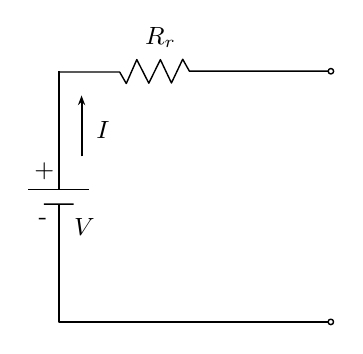
\begin{tikzpicture}[y=0.80pt, x=0.80pt, yscale=-\globalscale, xscale=\globalscale, inner sep=0pt, outer sep=0pt]
\path[draw=black,line join=round,line width=0.512pt] (0.3200,76.2640) -- (27.7628,76.2640);
\small


\path[draw=black,line join=round,line width=0.512pt] (7.2943,82.7528) -- (20.7883,82.7529);



\path[draw=black,line join=round,line width=0.512pt] (14.1449,76.2448) -- (14.1449,22.8468);



\path[draw=black,line join=round,line width=0.512pt] (135.8600,136.0210) -- (14.1449,136.0210) -- (14.1449,82.6234);



\path[draw=black,line join=round,line width=0.512pt] (135.8740,22.7108) -- (73.0453,22.7108) -- (70.0232,17.3162) -- (64.9397,28.0588) -- (59.9491,17.5021) -- (54.7105,28.1359) -- (49.2861,17.4866) -- (44.5437,28.2914) -- (41.5450,23.0911) -- (13.9128,23.0911);



\path[draw=black,line join=round,line width=0.512pt] (136.9300,134.7230) .. controls (137.6130,134.7230) and (138.1670,135.2770) .. (138.1670,135.9600) .. controls (138.1670,136.6430) and (137.6130,137.1970) .. (136.9300,137.1970) .. controls (136.2470,137.1970) and (135.6930,136.6430) .. (135.6930,135.9600) .. controls (135.6930,135.2770) and (136.2470,134.7230) .. (136.9300,134.7230) -- cycle;



\path[draw=black,line join=round,line width=0.512pt] (136.9590,21.4962) .. controls (137.6420,21.4962) and (138.1960,22.0499) .. (138.1960,22.7331) .. controls (138.1960,23.4163) and (137.6420,23.9701) .. (136.9590,23.9701) .. controls (136.2760,23.9701) and (135.7220,23.4163) .. (135.7220,22.7331) .. controls (135.7220,22.0499) and (136.2760,21.4962) .. (136.9590,21.4962) -- cycle;



\path[cm={{1.0,0.0,0.0,1.0,(3.0,72.0)}}] (0.0000,0.0000) node[above right] () {+};



\path[cm={{1.0,0.0,0.0,1.0,(5.0,92.0)}}] (0.0000,0.0000) node[above right] () {-};



\path[cm={{1.0,0.0,0.0,1.0,(21.0,97.0)}}] (0.0000,0.0000) node[above right] () {$V$};



\path[cm={{1.0,0.0,0.0,1.0,(53.0,12.0)}}] (0.0000,0.0000) node[above right] () {$R_r$};



\path[draw=black,line join=round,line width=0.512pt] (24.4663,61.1827) -- (24.4663,35.6490);



\path[fill=black,line join=round,line width=0.160pt] (22.6705,38.1118) -- (24.4135,36.5743) -- (26.0112,38.1047) -- (24.3349,33.6813) -- (22.6705,38.1118) -- cycle;



\path[cm={{1.0,0.0,0.0,1.0,(31.0,53.0)}}] (0.0000,0.0000) node[above right] () {$I$};




\end{tikzpicture}


  \caption[Equivalent electrical circuit for battery modeling with an internal resistance]{Equivalent electrical circuit for battery modeling with one resistor, representing the internal battery resistance.}
  \label{fig:rint}
  \efr
\end{figure}
Here, we propose a simplistic battery model to model a Li-ion battery of an aerial robot in flight, focusing on lesser complexity rather than accuracy. The battery SoC changes--when computations and motion generate a current to be drawn from the battery--according to the equation~\citep{zhang2018online,hasan2018exogenous}
\begin{equation}\label{eq:socevol}
  \dot{b}(y(t))=-I(y(t))/Q_c,
\end{equation}
where $Q_c\in\mathbb{R}$ is the battery constant nominal capacity measured in amperes per hour, $I(y(t))\in\mathbb{R}$ is the internal current that we derive later in this section, and $y(t)\in\mathbb{R}_{\geq 0}$ is a power drawn, i.e., the power needed for the computations and the motion. 
If we use the computations energy model in \fref{sec:comp-ener-model}{Section}, it is the power metric in \fref{def:comp-ener}{Definition} or the value of the measurement layer in \fref{def:measur-layer}{Definition} for each time step.

We propose a simplistic ECM with an internal resistance from the literature~\citep{mousavi2014various,hinz2019comparison,he2011evaluation} in \fref{fig:rint}{Figure}, sometimes termed the ``Rint'' model~\citep{hinz2019comparison,he2011evaluation}. The circuit models the battery simply as a perfect voltage source connected with a resistor $R_r\in\mathbb{R}$ measured in ohms, representing the internal battery resistance. The voltage $V\in\mathbb{R}$ measured in volts is the internal battery voltage, which depends on SoC~\citep{hasan2018exogenous} and can be retrieved from a battery data sheet~\citep{hinz2019comparison}, and $I$ is the current running through the circuit that depends on the power requirements of the load.

The voltage on the extremes of the ECM then respects 
\begin{equation}\label{eq:tocomb1}
  V_e=V-R_rI,
\end{equation}
where $V_e\in\mathbb{R}$ is the external battery voltage at the extremes of the circuit in \fref{fig:rint}{Figure}. If we assume that the voltage needed by the computations and motion is stable, let's call it $V_s\in\mathbb{R}$ and is measured in volts, and that the current required by the load (computations and motion) is $I_l$, we can write
\begin{equation}\label{eq:tocomb2}
  V_sI_l=V_eI,
\end{equation}
using simply Kirchhoff's circuit laws (the power into the load should exactly match the power out). Combining the \frefeqM{eq:tocomb1}{eq:tocomb2}, we obtain the quadratic expression $R_rI^2-VI+V_sI_l=0$, which leads to
\begin{equation}\label{eq:internal_curr}
  I(y(t))=\left(V-\sqrt{V^2-4R_ry(t)}\right)/(2R_r),
\end{equation}
where $I_l:=y(t)/V_s$ is the current of the load depending on the computations and motion power $y(t)$ at a given time instant $t$ in \frefeq{eq:socevol}. Furthermore, we take the negative solution of the quadratic expression: when $I_l$ is zero, $I$ should also be zero. With the internal current in \frefeq{eq:internal_curr} combined with the battery SoC in \frefeq{eq:socevol}, we can model how the computations and motion power trajectory $y(t)$ on $t\in\mathcal{T}:=[t_0,t_f]$ for given initial and final time instants ($t_0,t_f$ respectively) affects the battery. In one of our earlier intuitions~\citep{seewald2019coarse}, we expected a constant energy load to result in a better overall SoC compared to, e.g., a spiked one, even if the two have the same overall energy. The model above confirms this intuition. In \fref{fig:}{Figure}, we show the evolution of $I$ in \frefeq{eq:internal_curr} for a given linear load $I_l$ from zero to approximately one-third, assuming $V=V_s=R_r$ all one. The curve in the plot bends upwards for the plotted range: a line between two points will always be above the curve; it implies that a constant load is to be preferred compared to a load that repeatedly changes from high to low.

There are also more complex ECMs in the literature~\citep{hinz2019comparison,hasan2018exogenous}, which add additional elements to, e.g., account for the changes in the load current. One such ECM is the Thevenin model and the Thevenin-based model~\citep{chen2006accurate,hasan2018exogenous,hinz2019comparison,mousavi2014various,zhang2018online,salameh1992mathematical}\findex{Thevenin model}. 
\begin{figure}[h!]
  \sfr
  \centering
  \fontfamily{phv}\selectfont
  


\def \globalscale {.900000}
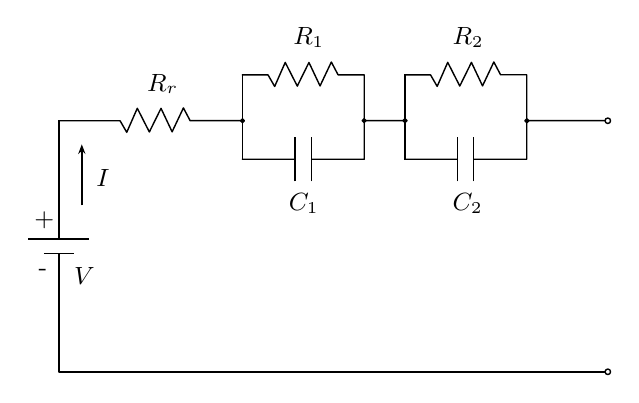
\begin{tikzpicture}[y=0.80pt, x=0.80pt, yscale=-\globalscale, xscale=\globalscale, inner sep=0pt, outer sep=0pt]
\small
\path[draw=black,line join=round,line width=0.512pt] (0.3200,96.5242) -- (27.8896,96.5242);



\path[draw=black,line join=round,line width=0.512pt] (7.3265,103.0430) -- (20.8829,103.0430);



\path[draw=black,line join=round,line width=0.512pt] (14.2088,96.5048) -- (14.2088,42.8600);



\path[draw=black,line join=round,line width=0.512pt] (260.9630,156.5580) -- (14.2088,156.5580) -- (14.2088,102.9130);



\path[draw=black,line join=round,line width=0.512pt] (260.8000,43.0793) -- (225.4320,43.0790);



\path[draw=black,line join=round,line width=0.512pt] (97.0029,43.0790) -- (73.3821,43.0790) -- (70.3453,37.3038) -- (65.2383,48.0961) -- (60.2246,37.4905) -- (54.9619,48.1735) -- (49.5124,37.4750) -- (44.7480,48.3298) -- (41.7355,43.1054) -- (13.9755,43.1054);



\path[draw=black,line join=round,line width=0.512pt] (262.0370,155.2530) .. controls (262.7240,155.2530) and (263.2800,155.8100) .. (263.2800,156.4960) .. controls (263.2800,157.1820) and (262.7240,157.7390) .. (262.0370,157.7390) .. controls (261.3510,157.7390) and (260.7950,157.1820) .. (260.7950,156.4960) .. controls (260.7950,155.8100) and (261.3510,155.2530) .. (262.0370,155.2530) -- cycle;



\path[draw=black,line join=round,line width=0.512pt] (262.0370,41.8587) .. controls (262.7240,41.8587) and (263.2800,42.4151) .. (263.2800,43.1014) .. controls (263.2800,43.7878) and (262.7240,44.3441) .. (262.0370,44.3441) .. controls (261.3510,44.3441) and (260.7950,43.7878) .. (260.7950,43.1014) .. controls (260.7950,42.4151) and (261.3510,41.8587) .. (262.0370,41.8587) -- cycle;



\path[cm={{1.0,0.0,0.0,1.0,(3.0,92.0)}}] (0.0000,0.0000) node[above right] () {+};



\path[cm={{1.0,0.0,0.0,1.0,(5.0,113.0)}}] (0.0000,0.0000) node[above right] () {-};



\path[cm={{1.0,0.0,0.0,1.0,(21.0,117.0)}}] (0.0000,0.0000) node[above right] () {$V$};



\path[cm={{1.0,0.0,0.0,1.0,(54.0,31.0)}}] (0.0000,0.0000) node[above right] () {$R_r$};



\path[draw=black,line join=round,line width=0.512pt] (24.5779,81.3732) -- (24.5779,55.7215);



\path[fill=black,line join=round,line width=0.160pt] (22.7737,58.1955) -- (24.5247,56.6509) -- (26.1298,58.1885) -- (24.4458,53.7447) -- (22.7737,58.1955) -- cycle;



\path[cm={{1.0,0.0,0.0,1.0,(31.0,73.0)}}] (0.0000,0.0000) node[above right] () {$I$};



\path[draw=black,line join=round,line width=0.512pt] (97.0247,60.6763) -- (97.0247,22.1411);



\path[draw=black,line join=round,line width=0.512pt] (96.7722,60.5081) -- (120.7290,60.5085);



\path[draw=black,line join=round,line width=0.512pt] (128.0790,60.5086) -- (152.0390,60.5091) -- (152.0390,22.3621) -- (140.1990,22.3602) -- (137.1630,16.5849) -- (132.0560,27.3773) -- (127.0420,16.7717) -- (121.7800,27.4547) -- (116.3300,16.7562) -- (111.5660,27.6108) -- (108.5530,22.3864) -- (96.7913,22.3869);



\path[draw=black,line join=round,line width=0.512pt] (120.7490,70.4544) -- (120.7490,50.4562);



\path[draw=black,line join=round,line width=0.512pt] (128.0730,70.4544) -- (128.0730,50.4562);



\path[draw=black,line join=round,line width=0.512pt] (170.4000,43.0569) -- (152.1120,43.0573);



\path[draw=black,line join=round,line width=0.512pt] (170.4220,60.6542) -- (170.4220,22.1190);



\path[draw=black,line join=round,line width=0.512pt] (170.1690,60.4860) -- (194.1260,60.4864);



\path[draw=black,line join=round,line width=0.512pt] (201.4760,60.4865) -- (225.4360,60.4870) -- (225.4360,22.3400) -- (213.5960,22.3381) -- (210.5600,16.5628) -- (205.4530,27.3552) -- (200.4400,16.7496) -- (195.1770,27.4326) -- (189.7270,16.7341) -- (184.9630,27.5887) -- (181.9510,22.3643) -- (170.1890,22.3648);



\path[draw=black,line join=round,line width=0.512pt] (194.1470,70.4323) -- (194.1470,50.4341);



\path[draw=black,line join=round,line width=0.512pt] (201.4700,70.4323) -- (201.4700,50.4341);



\path[draw=black,fill=black,line join=round,line width=0.512pt] (225.4900,42.2159) .. controls (225.9770,42.2159) and (226.3720,42.6107) .. (226.3720,43.0978) .. controls (226.3720,43.5850) and (225.9770,43.9799) .. (225.4900,43.9799) .. controls (225.0030,43.9799) and (224.6080,43.5850) .. (224.6080,43.0978) .. controls (224.6080,42.6107) and (225.0030,42.2159) .. (225.4900,42.2159) -- cycle;



\path[draw=black,fill=black,line join=round,line width=0.512pt] (170.4530,42.1766) .. controls (170.9400,42.1766) and (171.3350,42.5714) .. (171.3350,43.0585) .. controls (171.3350,43.5457) and (170.9400,43.9406) .. (170.4530,43.9406) .. controls (169.9660,43.9406) and (169.5710,43.5457) .. (169.5710,43.0585) .. controls (169.5710,42.5714) and (169.9660,42.1766) .. (170.4530,42.1766) -- cycle;



\path[draw=black,fill=black,line join=round,line width=0.512pt] (151.9710,42.1544) .. controls (152.4580,42.1544) and (152.8530,42.5491) .. (152.8530,43.0363) .. controls (152.8530,43.5235) and (152.4580,43.9184) .. (151.9710,43.9184) .. controls (151.4830,43.9184) and (151.0890,43.5235) .. (151.0890,43.0363) .. controls (151.0890,42.5491) and (151.4830,42.1544) .. (151.9710,42.1544) -- cycle;



\path[draw=black,fill=black,line join=round,line width=0.512pt] (97.0363,42.2150) .. controls (97.5234,42.2150) and (97.9183,42.6099) .. (97.9183,43.0971) .. controls (97.9183,43.5843) and (97.5234,43.9792) .. (97.0363,43.9792) .. controls (96.5491,43.9792) and (96.1542,43.5843) .. (96.1542,43.0971) .. controls (96.1542,42.6099) and (96.5491,42.2150) .. (97.0363,42.2150) -- cycle;



\path[cm={{1.0,0.0,0.0,1.0,(120.0,10.0)}}] (0.0000,0.0000) node[above right] () {$R_1$};



\path[cm={{1.0,0.0,0.0,1.0,(192.0,10.0)}}] (0.0000,0.0000) node[above right] () {$R_2$};



\path[cm={{1.0,0.0,0.0,1.0,(118.0,85.0)}}] (0.0000,0.0000) node[above right] () {$C_1$};



\path[cm={{1.0,0.0,0.0,1.0,(192.0,85.0)}}] (0.0000,0.0000) node[above right] () {$C_2$};




\end{tikzpicture}


  \caption[Thevenin-based equivalent electrical circuit for battery modeling]{Thevenin-based equivalent electrical circuit for battery modeling with one resistor and two RC internal elements. The two elements add some complexity, making the model able to account for changes in the load current.}
  \label{fig:thevenin}
  \efr
\end{figure}
Sometimes termed the dual-polarization model~\citep{he2011evaluation}, we illustrate the ECM in \fref{fig:thevenin}{Figure}. It models further details, such as the short-term transient behavior with the first RC element ($R_1,C_1$) and the long-term transient behavior with the second RC element ($R_2,C_2$)~\citep{hinz2019comparison}. It is particularly suitable to model the polarization characteristic of Li-ion battery cells~\citep{he2011evaluation}.

\subsection{Battery model in the {\tt powprofiler} tool}
\label{sec:batmod-circuit}

The \powprof{} tool allows automated battery modeling and directly derives battery SoC for each measurement layer in \fref{sec:measurement-layer}{Section}. Indeed in \fref{def:measur-layer}{Definition}, the function $\mathbf{g}$ returns a triplet of values, including the SoC. For the predictive layer in \fref{def:comp-ener}{Definition} in \fref{sec:predictive-layer}{Section}, the tool similarly outputs the SoC for a given configuration of parameters and energy sensor or other energy measuring device. To this end, it implements the simplistic equivalent electrical circuit in \fref{fig:rint}{Figure} from the literature~\citep{mousavi2014various,hinz2019comparison,he2011evaluation}, with the class {\small\tt soc\_1resistor}, where the constructor accepts in input the parameters $I_l,V,R_r,V_s$ and $Q_c$ that we discussed in \fref{sec:batmod-circuit}{Section}. The current load $I_l$ is expressed via the data type {\small\tt pathn} in \fref{sec:powprof}{Section}. One can implement a similar battery model, e.g., the Thevenin-based ECM in \fref{fig:thevenin}{Figure}, by simply inheriting from class {\small\tt first\_derivative} the function {\small\tt get\_value}. It returns the modeled battery SoC at the next time instant from an independent variable, i.e., time, and a dependent variable represented via the data type {\small\tt soc\_1resistor} in \fref{sec:powprof}{Section}.

Internally, the tool implements a numerical simulator based on the Runge-Kutta methods\findex{Runge-Kutta methods} for numerical integration\findex{numerical integration} in \fref{sec:rk4}{Section}. One can then personalize the size of the integration step $h\in\mathbb{R}_{>0}$ via the property {\small\tt h} in the configuration specification in \fref{sec:conf-spec}{Section} (a typical practical value of such property is, e.g., one hundredth). The tool first derives a model for the power and energy and later numerically simulates the battery model via the equivalent electrical circuit in \fref{fig:rint}{Figure} adjoining the battery SoC.


%%%%%%%%%%%%%%%%%%%%%%%%%%%%%%%%%%%%
\section{Energy Model of the Motion}
\label{sec:mot-ener-model}

In this section, we implement a model for the motion of aerial robots in coverage path planning (\Gls{acr:cpp})\findex{coverage path planning}. We first derive a differential periodic energy model and provide a formal proof in \fref{sec:deriv}{Section}. This model server to model the motion. We enhance the model with the path and computations parameters in \fref{sec:nom-cont}{Section}, to predict the energy consumption of a given configuration of parameters. We explain how we convert the parameters into actual energy consumption in \fref{sec:merging}{Section}, and discuss the model's behavior for aperiodic power evolutions in \fref{sec:non-perio}{Section}.

Let us suppose the aerial robot is operating in an autonomous scenario, planning the coverage and scheduling some computations for detections and encryption in \fref{sec:flight-plan}{Section}. 
\begin{figure}[h!]
  \sfr
  \centering
  \footnotesize
  \fontfamily{phv}\selectfont
  
\definecolor{ca0a0a4}{RGB}{160,160,164}


\def \globalscale {1.000000}
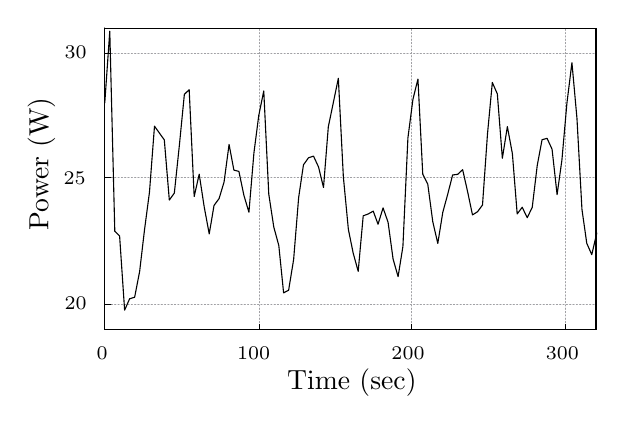
\begin{tikzpicture}[y=0.80pt, x=0.80pt, yscale=-.7*\globalscale, xscale=.9*\globalscale, inner sep=0pt, outer sep=0pt]
\begin{scope}[draw=black,line join=bevel,line cap=rect,even odd rule,line width=0.800pt]
  \begin{scope}[cm={{1.0,0.0,0.0,1.0,(0.0,0.0)}},draw=black,line join=bevel,line cap=rect,line width=0.800pt]
  \end{scope}
  \begin{scope}[cm={{1.00625,0.0,0.0,1.00625,(0.0,0.0)}},draw=black,line join=bevel,line cap=rect,line width=0.800pt]
  \end{scope}
  \begin{scope}[cm={{1.00625,0.0,0.0,1.00625,(0.0,0.0)}},draw=ca0a0a4,dash pattern=on 0.40pt off 0.80pt,line join=round,line cap=round,line width=0.400pt]
    \path[draw] (53.5000,192.5000) -- (298.5000,192.5000);



  \end{scope}
  \begin{scope}[cm={{1.00625,0.0,0.0,1.00625,(0.0,0.0)}},draw=black,line join=round,line cap=round,line width=0.400pt]
    \path[draw] (53.5000,192.5000) -- (56.5000,192.5000);



  \end{scope}
  \begin{scope}[cm={{1.00625,0.0,0.0,1.00625,(0.0,0.0)}},draw=black,line join=bevel,line cap=rect,line width=0.800pt]
  \end{scope}
  \begin{scope}[cm={{1.00625,0.0,0.0,1.00625,(36.7281,197.225)}},draw=black,line join=bevel,line cap=rect,line width=0.800pt]
  \end{scope}
  \begin{scope}[cm={{1.00625,0.0,0.0,1.00625,(36.7281,197.225)}},draw=black,line join=bevel,line cap=rect,line width=0.800pt]
  \end{scope}
  \begin{scope}[cm={{1.00625,0.0,0.0,1.00625,(36.7281,197.225)}},draw=black,line join=bevel,line cap=rect,line width=0.800pt]
  \end{scope}
  \begin{scope}[cm={{1.00625,0.0,0.0,1.00625,(36.7281,197.225)}},draw=black,line join=bevel,line cap=rect,line width=0.800pt]
  \end{scope}
  \begin{scope}[cm={{1.00625,0.0,0.0,1.00625,(36.7281,197.225)}},draw=black,line join=bevel,line cap=rect,line width=0.800pt]
  \end{scope}
  \begin{scope}[cm={{1.00625,0.0,0.0,1.00625,(33.7281,197.225)}},draw=black,line join=bevel,line cap=rect,line width=0.800pt]
    \path[fill=black] (0.0000,0.0000) node[above right] () {\scriptsize 20};



  \end{scope}
  \begin{scope}[cm={{1.00625,0.0,0.0,1.00625,(36.7281,197.225)}},draw=black,line join=bevel,line cap=rect,line width=0.800pt]
  \end{scope}
  \begin{scope}[cm={{1.00625,0.0,0.0,1.00625,(0.0,0.0)}},draw=black,line join=bevel,line cap=rect,line width=0.800pt]
  \end{scope}
  \begin{scope}[cm={{1.00625,0.0,0.0,1.00625,(0.0,0.0)}},draw=ca0a0a4,dash pattern=on 0.40pt off 0.80pt,line join=round,line cap=round,line width=0.400pt]
    \path[draw] (53.5000,111.5000) -- (298.5000,111.5000);



  \end{scope}
  \begin{scope}[cm={{1.00625,0.0,0.0,1.00625,(0.0,0.0)}},draw=black,line join=round,line cap=round,line width=0.400pt]
    \path[draw] (53.5000,111.5000) -- (56.5000,111.5000);



  \end{scope}
  \begin{scope}[cm={{1.00625,0.0,0.0,1.00625,(0.0,0.0)}},draw=black,line join=bevel,line cap=rect,line width=0.800pt]
  \end{scope}
  \begin{scope}[cm={{1.00625,0.0,0.0,1.00625,(37.2313,116.725)}},draw=black,line join=bevel,line cap=rect,line width=0.800pt]
  \end{scope}
  \begin{scope}[cm={{1.00625,0.0,0.0,1.00625,(37.2313,116.725)}},draw=black,line join=bevel,line cap=rect,line width=0.800pt]
  \end{scope}
  \begin{scope}[cm={{1.00625,0.0,0.0,1.00625,(37.2313,116.725)}},draw=black,line join=bevel,line cap=rect,line width=0.800pt]
  \end{scope}
  \begin{scope}[cm={{1.00625,0.0,0.0,1.00625,(37.2313,116.725)}},draw=black,line join=bevel,line cap=rect,line width=0.800pt]
  \end{scope}
  \begin{scope}[cm={{1.00625,0.0,0.0,1.00625,(37.2313,116.725)}},draw=black,line join=bevel,line cap=rect,line width=0.800pt]
  \end{scope}
  \begin{scope}[cm={{1.00625,0.0,0.0,1.00625,(33.2313,116.725)}},draw=black,line join=bevel,line cap=rect,line width=0.800pt]
    \path[fill=black] (0.0000,0.0000) node[above right] () {\scriptsize 25};



  \end{scope}
  \begin{scope}[cm={{1.00625,0.0,0.0,1.00625,(37.2313,116.725)}},draw=black,line join=bevel,line cap=rect,line width=0.800pt]
  \end{scope}
  \begin{scope}[cm={{1.00625,0.0,0.0,1.00625,(0.0,0.0)}},draw=black,line join=bevel,line cap=rect,line width=0.800pt]
  \end{scope}
  \begin{scope}[cm={{1.00625,0.0,0.0,1.00625,(0.0,0.0)}},draw=ca0a0a4,dash pattern=on 0.40pt off 0.80pt,line join=round,line cap=round,line width=0.400pt]
    \path[draw] (53.5000,31.5000) -- (298.5000,31.5000);



  \end{scope}
  \begin{scope}[cm={{1.00625,0.0,0.0,1.00625,(0.0,0.0)}},draw=black,line join=round,line cap=round,line width=0.400pt]
    \path[draw] (53.5000,31.5000) -- (56.5000,31.5000);



  \end{scope}
  \begin{scope}[cm={{1.00625,0.0,0.0,1.00625,(0.0,0.0)}},draw=black,line join=bevel,line cap=rect,line width=0.800pt]
  \end{scope}
  \begin{scope}[cm={{1.00625,0.0,0.0,1.00625,(36.7281,35.2188)}},draw=black,line join=bevel,line cap=rect,line width=0.800pt]
  \end{scope}
  \begin{scope}[cm={{1.00625,0.0,0.0,1.00625,(36.7281,35.2188)}},draw=black,line join=bevel,line cap=rect,line width=0.800pt]
  \end{scope}
  \begin{scope}[cm={{1.00625,0.0,0.0,1.00625,(36.7281,35.2188)}},draw=black,line join=bevel,line cap=rect,line width=0.800pt]
  \end{scope}
  \begin{scope}[cm={{1.00625,0.0,0.0,1.00625,(36.7281,35.2188)}},draw=black,line join=bevel,line cap=rect,line width=0.800pt]
  \end{scope}
  \begin{scope}[cm={{1.00625,0.0,0.0,1.00625,(36.7281,35.2188)}},draw=black,line join=bevel,line cap=rect,line width=0.800pt]
  \end{scope}
  \begin{scope}[cm={{1.00625,0.0,0.0,1.00625,(33.7281,35.2188)}},draw=black,line join=bevel,line cap=rect,line width=0.800pt]
    \path[fill=black] (0.0000,0.0000) node[above right] () {\scriptsize 30};



  \end{scope}
  \begin{scope}[cm={{1.00625,0.0,0.0,1.00625,(36.7281,35.2188)}},draw=black,line join=bevel,line cap=rect,line width=0.800pt]
  \end{scope}
  \begin{scope}[cm={{1.00625,0.0,0.0,1.00625,(0.0,0.0)}},draw=black,line join=bevel,line cap=rect,line width=0.800pt]
  \end{scope}
  \begin{scope}[cm={{1.00625,0.0,0.0,1.00625,(0.0,0.0)}},draw=ca0a0a4,dash pattern=on 0.40pt off 0.80pt,line join=round,line cap=round,line width=0.400pt]
    \path[draw] (53.5000,208.5000) -- (53.5000,15.5000);



  \end{scope}
  \begin{scope}[cm={{1.00625,0.0,0.0,1.00625,(0.0,0.0)}},draw=black,line join=round,line cap=round,line width=0.400pt]
    \path[draw] (53.5000,208.5000) -- (53.5000,205.5000);



  \end{scope}
  \begin{scope}[cm={{1.00625,0.0,0.0,1.00625,(0.0,0.0)}},draw=black,line join=bevel,line cap=rect,line width=0.800pt]
  \end{scope}
  \begin{scope}[cm={{1.00625,0.0,0.0,1.00625,(49.8094,221.375)}},draw=black,line join=bevel,line cap=rect,line width=0.800pt]
  \end{scope}
  \begin{scope}[cm={{1.00625,0.0,0.0,1.00625,(49.8094,221.375)}},draw=black,line join=bevel,line cap=rect,line width=0.800pt]
  \end{scope}
  \begin{scope}[cm={{1.00625,0.0,0.0,1.00625,(49.8094,221.375)}},draw=black,line join=bevel,line cap=rect,line width=0.800pt]
  \end{scope}
  \begin{scope}[cm={{1.00625,0.0,0.0,1.00625,(49.8094,221.375)}},draw=black,line join=bevel,line cap=rect,line width=0.800pt]
  \end{scope}
  \begin{scope}[cm={{1.00625,0.0,0.0,1.00625,(49.8094,221.375)}},draw=black,line join=bevel,line cap=rect,line width=0.800pt]
  \end{scope}
  \begin{scope}[cm={{1.00625,0.0,0.0,1.00625,(49.8094,229.375)}},draw=black,line join=bevel,line cap=rect,line width=0.800pt]
    \path[fill=black] (0.0000,0.0000) node[above right] () {\scriptsize 0};



  \end{scope}
  \begin{scope}[cm={{1.00625,0.0,0.0,1.00625,(49.8094,221.375)}},draw=black,line join=bevel,line cap=rect,line width=0.800pt]
  \end{scope}
  \begin{scope}[cm={{1.00625,0.0,0.0,1.00625,(0.0,0.0)}},draw=black,line join=bevel,line cap=rect,line width=0.800pt]
  \end{scope}
  \begin{scope}[cm={{1.00625,0.0,0.0,1.00625,(0.0,0.0)}},draw=ca0a0a4,dash pattern=on 0.40pt off 0.80pt,line join=round,line cap=round,line width=0.400pt]
    \path[draw] (130.5000,208.5000) -- (130.5000,15.5000);



  \end{scope}
  \begin{scope}[cm={{1.00625,0.0,0.0,1.00625,(0.0,0.0)}},draw=black,line join=round,line cap=round,line width=0.400pt]
    \path[draw] (130.5000,208.5000) -- (130.5000,205.5000);



  \end{scope}
  \begin{scope}[cm={{1.00625,0.0,0.0,1.00625,(0.0,0.0)}},draw=black,line join=bevel,line cap=rect,line width=0.800pt]
  \end{scope}
  \begin{scope}[cm={{1.00625,0.0,0.0,1.00625,(120.247,221.375)}},draw=black,line join=bevel,line cap=rect,line width=0.800pt]
  \end{scope}
  \begin{scope}[cm={{1.00625,0.0,0.0,1.00625,(120.247,221.375)}},draw=black,line join=bevel,line cap=rect,line width=0.800pt]
  \end{scope}
  \begin{scope}[cm={{1.00625,0.0,0.0,1.00625,(120.247,221.375)}},draw=black,line join=bevel,line cap=rect,line width=0.800pt]
  \end{scope}
  \begin{scope}[cm={{1.00625,0.0,0.0,1.00625,(120.247,221.375)}},draw=black,line join=bevel,line cap=rect,line width=0.800pt]
  \end{scope}
  \begin{scope}[cm={{1.00625,0.0,0.0,1.00625,(120.247,221.375)}},draw=black,line join=bevel,line cap=rect,line width=0.800pt]
  \end{scope}
  \begin{scope}[cm={{1.00625,0.0,0.0,1.00625,(120.247,229.375)}},draw=black,line join=bevel,line cap=rect,line width=0.800pt]
    \path[fill=black] (0.0000,0.0000) node[above right] () {\scriptsize 100};



  \end{scope}
  \begin{scope}[cm={{1.00625,0.0,0.0,1.00625,(120.247,221.375)}},draw=black,line join=bevel,line cap=rect,line width=0.800pt]
  \end{scope}
  \begin{scope}[cm={{1.00625,0.0,0.0,1.00625,(0.0,0.0)}},draw=black,line join=bevel,line cap=rect,line width=0.800pt]
  \end{scope}
  \begin{scope}[cm={{1.00625,0.0,0.0,1.00625,(0.0,0.0)}},draw=ca0a0a4,dash pattern=on 0.40pt off 0.80pt,line join=round,line cap=round,line width=0.400pt]
    \path[draw] (206.5000,208.5000) -- (206.5000,15.5000);



  \end{scope}
  \begin{scope}[cm={{1.00625,0.0,0.0,1.00625,(0.0,0.0)}},draw=black,line join=round,line cap=round,line width=0.400pt]
    \path[draw] (206.5000,208.5000) -- (206.5000,205.5000);



  \end{scope}
  \begin{scope}[cm={{1.00625,0.0,0.0,1.00625,(0.0,0.0)}},draw=black,line join=bevel,line cap=rect,line width=0.800pt]
  \end{scope}
  \begin{scope}[cm={{1.00625,0.0,0.0,1.00625,(197.728,221.375)}},draw=black,line join=bevel,line cap=rect,line width=0.800pt]
  \end{scope}
  \begin{scope}[cm={{1.00625,0.0,0.0,1.00625,(197.728,221.375)}},draw=black,line join=bevel,line cap=rect,line width=0.800pt]
  \end{scope}
  \begin{scope}[cm={{1.00625,0.0,0.0,1.00625,(197.728,221.375)}},draw=black,line join=bevel,line cap=rect,line width=0.800pt]
  \end{scope}
  \begin{scope}[cm={{1.00625,0.0,0.0,1.00625,(197.728,221.375)}},draw=black,line join=bevel,line cap=rect,line width=0.800pt]
  \end{scope}
  \begin{scope}[cm={{1.00625,0.0,0.0,1.00625,(197.728,221.375)}},draw=black,line join=bevel,line cap=rect,line width=0.800pt]
  \end{scope}
  \begin{scope}[cm={{1.00625,0.0,0.0,1.00625,(197.728,229.375)}},draw=black,line join=bevel,line cap=rect,line width=0.800pt]
    \path[fill=black] (0.0000,0.0000) node[above right] () {\scriptsize 200};



  \end{scope}
  \begin{scope}[cm={{1.00625,0.0,0.0,1.00625,(197.728,221.375)}},draw=black,line join=bevel,line cap=rect,line width=0.800pt]
  \end{scope}
  \begin{scope}[cm={{1.00625,0.0,0.0,1.00625,(0.0,0.0)}},draw=black,line join=bevel,line cap=rect,line width=0.800pt]
  \end{scope}
  \begin{scope}[cm={{1.00625,0.0,0.0,1.00625,(0.0,0.0)}},draw=ca0a0a4,dash pattern=on 0.40pt off 0.80pt,line join=round,line cap=round,line width=0.400pt]
    \path[draw] (283.5000,208.5000) -- (283.5000,21.5000) -- (283.5000,21.5000) -- (283.5000,15.5000);



  \end{scope}
  \begin{scope}[cm={{1.00625,0.0,0.0,1.00625,(0.0,0.0)}},draw=black,line join=round,line cap=round,line width=0.400pt]
    \path[draw] (283.5000,208.5000) -- (283.5000,205.5000);



  \end{scope}
  \begin{scope}[cm={{1.00625,0.0,0.0,1.00625,(0.0,0.0)}},draw=black,line join=bevel,line cap=rect,line width=0.800pt]
  \end{scope}
  \begin{scope}[cm={{1.00625,0.0,0.0,1.00625,(275.209,221.375)}},draw=black,line join=bevel,line cap=rect,line width=0.800pt]
  \end{scope}
  \begin{scope}[cm={{1.00625,0.0,0.0,1.00625,(275.209,221.375)}},draw=black,line join=bevel,line cap=rect,line width=0.800pt]
  \end{scope}
  \begin{scope}[cm={{1.00625,0.0,0.0,1.00625,(275.209,221.375)}},draw=black,line join=bevel,line cap=rect,line width=0.800pt]
  \end{scope}
  \begin{scope}[cm={{1.00625,0.0,0.0,1.00625,(275.209,221.375)}},draw=black,line join=bevel,line cap=rect,line width=0.800pt]
  \end{scope}
  \begin{scope}[cm={{1.00625,0.0,0.0,1.00625,(275.209,221.375)}},draw=black,line join=bevel,line cap=rect,line width=0.800pt]
  \end{scope}
  \begin{scope}[cm={{1.00625,0.0,0.0,1.00625,(275.209,229.375)}},draw=black,line join=bevel,line cap=rect,line width=0.800pt]
    \path[fill=black] (0.0000,0.0000) node[above right] () {\scriptsize 300};



  \end{scope}
  \begin{scope}[cm={{1.00625,0.0,0.0,1.00625,(275.209,221.375)}},draw=black,line join=bevel,line cap=rect,line width=0.800pt]
  \end{scope}
  \begin{scope}[cm={{1.00625,0.0,0.0,1.00625,(0.0,0.0)}},draw=black,line join=bevel,line cap=rect,line width=0.800pt]
  \end{scope}
  \begin{scope}[cm={{1.00625,0.0,0.0,1.00625,(0.0,0.0)}},draw=black,line join=round,line cap=round,line width=0.400pt]
    \path[draw] (53.5000,15.5000) -- (53.5000,208.5000) -- (298.5000,208.5000) -- (298.5000,15.5000) -- (53.5000,15.5000);



  \end{scope}
  \begin{scope}[cm={{1.00625,0.0,0.0,1.00625,(0.0,0.0)}},draw=black,line join=bevel,line cap=rect,line width=0.800pt]
  \end{scope}
  \begin{scope}[cm={{0.0,-1.00625,1.00625,0.0,(23.1438,138.863)}},draw=black,line join=bevel,line cap=rect,line width=0.800pt]
  \end{scope}
  \begin{scope}[cm={{0.0,-1.00625,1.00625,0.0,(23.1438,138.863)}},draw=black,line join=bevel,line cap=rect,line width=0.800pt]
  \end{scope}
  \begin{scope}[cm={{0.0,-1.00625,1.00625,0.0,(23.1438,138.863)}},draw=black,line join=bevel,line cap=rect,line width=0.800pt]
  \end{scope}
  \begin{scope}[cm={{0.0,-1.00625,1.00625,0.0,(23.1438,138.863)}},draw=black,line join=bevel,line cap=rect,line width=0.800pt]
  \end{scope}
  \begin{scope}[cm={{0.0,-1.00625,1.00625,0.0,(23.1438,138.863)}},draw=black,line join=bevel,line cap=rect,line width=0.800pt]
  \end{scope}
  \begin{scope}[cm={{0.0,-1.00625,1.00625,0.0,(15.1438,145.863)}},draw=black,line join=bevel,line cap=rect,line width=0.800pt]
    \path[fill=black] (0.0000,0.0000) node[above right] () {\rotatebox{90}{Power (W)}};



  \end{scope}
  \begin{scope}[cm={{0.0,-1.00625,1.00625,0.0,(23.1438,138.863)}},draw=black,line join=bevel,line cap=rect,line width=0.800pt]
  \end{scope}
  \begin{scope}[cm={{1.00625,0.0,0.0,1.00625,(147.416,235.463)}},draw=black,line join=bevel,line cap=rect,line width=0.800pt]
  \end{scope}
  \begin{scope}[cm={{1.00625,0.0,0.0,1.00625,(147.416,235.463)}},draw=black,line join=bevel,line cap=rect,line width=0.800pt]
  \end{scope}
  \begin{scope}[cm={{1.00625,0.0,0.0,1.00625,(147.416,235.463)}},draw=black,line join=bevel,line cap=rect,line width=0.800pt]
  \end{scope}
  \begin{scope}[cm={{1.00625,0.0,0.0,1.00625,(147.416,235.463)}},draw=black,line join=bevel,line cap=rect,line width=0.800pt]
  \end{scope}
  \begin{scope}[cm={{1.00625,0.0,0.0,1.00625,(147.416,235.463)}},draw=black,line join=bevel,line cap=rect,line width=0.800pt]
  \end{scope}
  \begin{scope}[cm={{1.00625,0.0,0.0,1.00625,(145.416,253.463)}},draw=black,line join=bevel,line cap=rect,line width=0.800pt]
    \path[fill=black] (0.0000,0.0000) node[above right] () {Time (sec)};



  \end{scope}
  \begin{scope}[cm={{1.00625,0.0,0.0,1.00625,(147.416,235.463)}},draw=black,line join=bevel,line cap=rect,line width=0.800pt]
  \end{scope}
  \begin{scope}[cm={{1.00625,0.0,0.0,1.00625,(0.0,0.0)}},draw=black,line join=bevel,line cap=rect,line width=0.800pt]
  \end{scope}
  \begin{scope}[cm={{1.00625,0.0,0.0,1.00625,(0.0,0.0)}},draw=black,line join=bevel,line cap=rect,line width=0.800pt]
  \end{scope}
  \begin{scope}[cm={{1.00625,0.0,0.0,1.00625,(0.0,0.0)}},draw=black,line join=bevel,line cap=rect,line width=0.800pt]
  \end{scope}
  \begin{scope}[cm={{1.00625,0.0,0.0,1.00625,(0.0,0.0)}},draw=black,line join=round,line cap=round,line width=0.400pt]
    \path[draw] (53.5000,63.4000) -- (53.5000,63.4000) -- (56.0000,17.4000) -- (58.5000,145.7000) -- (60.9000,148.7000) -- (63.4000,196.3000) -- (65.9000,189.0000) -- (68.4000,188.0000) -- (70.9000,171.4000) -- (73.3000,145.0000) -- (75.8000,120.6000) -- (78.3000,78.3000) -- (80.8000,82.8000) -- (83.2000,87.1000) -- (85.7000,125.7000) -- (88.2000,121.2000) -- (90.7000,90.7000) -- (93.2000,57.9000) -- (95.6000,54.9000) -- (98.1000,123.4000) -- (100.6000,109.1000) -- (103.1000,130.1000) -- (105.6000,147.4000) -- (108.0000,129.1000) -- (110.5000,124.8000) -- (113.0000,114.1000) -- (115.5000,90.0000) -- (117.9000,106.5000) -- (120.4000,107.3000) -- (122.9000,122.7000) -- (125.4000,133.5000) -- (127.9000,95.4000) -- (130.3000,71.5000) -- (132.8000,55.7000) -- (135.3000,121.9000) -- (137.8000,143.0000) -- (140.3000,154.8000) -- (142.7000,185.2000) -- (145.2000,183.5000) -- (147.7000,163.8000) -- (150.2000,124.1000) -- (152.6000,103.1000) -- (155.1000,98.6000) -- (157.6000,97.5000) -- (160.1000,104.4000) -- (162.6000,117.6000) -- (165.0000,78.7000) -- (167.5000,63.2000) -- (170.0000,47.6000) -- (172.5000,110.8000) -- (175.0000,144.5000) -- (177.4000,159.7000) -- (179.9000,171.4000) -- (182.4000,135.8000) -- (184.9000,134.6000) -- (187.4000,132.8000) -- (189.8000,141.2000) -- (192.3000,130.7000) -- (194.8000,139.9000) -- (197.3000,163.5000) -- (199.8000,174.8000) -- (202.2000,155.5000) -- (204.7000,85.8000) -- (207.2000,61.1000) -- (209.7000,48.1000) -- (212.1000,109.1000) -- (214.6000,115.5000) -- (217.1000,139.6000) -- (219.6000,153.5000) -- (222.1000,133.5000) -- (224.5000,122.2000) -- (227.0000,109.6000) -- (229.5000,109.2000) -- (232.0000,106.2000) -- (234.5000,120.5000) -- (236.9000,135.2000) -- (239.4000,133.2000) -- (241.9000,128.9000) -- (244.4000,83.1000) -- (246.8000,50.3000) -- (249.3000,57.6000) -- (251.8000,98.9000) -- (254.3000,78.6000) -- (256.8000,95.9000) -- (259.2000,134.6000) -- (261.7000,130.3000) -- (264.2000,137.0000) -- (266.7000,130.4000) -- (269.2000,103.5000) -- (271.6000,87.0000) -- (274.1000,86.1000) -- (276.6000,93.1000) -- (279.1000,122.2000) -- (281.5000,100.1000) -- (284.0000,63.6000) -- (286.5000,37.6000) -- (289.0000,73.1000) -- (291.5000,131.6000) -- (293.9000,153.4000) -- (296.4000,160.7000) -- (298.9000,146.8000);



  \end{scope}
  \begin{scope}[cm={{1.00625,0.0,0.0,1.00625,(0.0,0.0)}},draw=black,line join=bevel,line cap=rect,line width=0.800pt]
  \end{scope}
  \begin{scope}[cm={{1.00625,0.0,0.0,1.00625,(0.0,0.0)}},draw=black,line join=bevel,line cap=rect,line width=0.800pt]
  \end{scope}
  \begin{scope}[cm={{1.00625,0.0,0.0,1.00625,(0.0,0.0)}},draw=black,line join=round,line cap=round,line width=0.400pt]
    \path[draw] (53.5000,15.5000) -- (53.5000,208.5000) -- (298.5000,208.5000) -- (298.5000,15.5000) -- (53.5000,15.5000);



  \end{scope}
  \begin{scope}[cm={{1.00625,0.0,0.0,1.00625,(0.0,0.0)}},draw=black,line join=bevel,line cap=rect,line width=0.800pt]
  \end{scope}
  \begin{scope}[cm={{1.0,0.0,0.0,1.0,(0.0,0.0)}},draw=black,line join=bevel,line cap=rect,line width=0.800pt]
  \end{scope}
\end{scope}

\end{tikzpicture}


  \caption[Power evolution data of an aerial robot in coverage planning]{Empirical energy data of the aerial robot in \fref{fig:plot2}{Figure} in coverage planning. The data shows that the energy signal is periodic over time as the fixed-wing aerial robot reiterates a set of paths.}
  \label{fig:energy-1}
  \efr
\end{figure}
It expectedly iterates some paths (the primitive paths) for CPP and schedules the computations periodically, as we outlined in \fref{sec:outline}{Section}, and further backed with the concept of primitive paths in \fref{def:primitive}{Definition}. Since the paths and tasks are periodically iterated over time, we expect the energy to evolve similarly. This assumption is further supported by our previous contribution on the topic~\citep{seewald2020mechanical}, showing that a Fourier series of a given order can model the energy of the aerial robot (in the contribution, we used the order three). We will ease the assumption of the periodic evolution in practice to periodic with disturbance or aperiodic evolutions in \fref{sec:non-perio}{Section}. 
\begin{figure}[h!]
  \sfr
  \centering
  \footnotesize
  \fontfamily{phv}\selectfont
  
\definecolor{ca0a0a4}{RGB}{160,160,164}


\def \globalscale {1.000000}
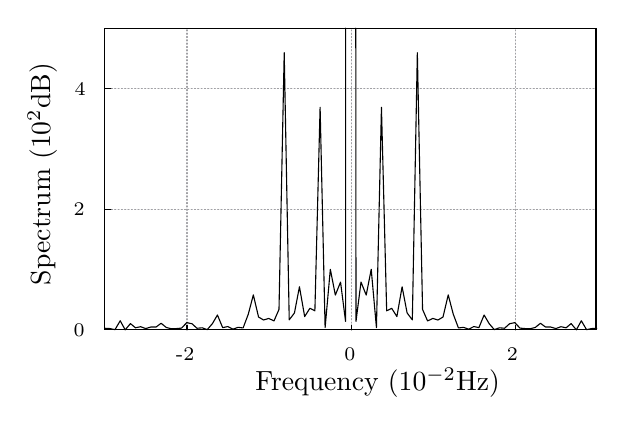
\begin{tikzpicture}[y=0.80pt, x=0.80pt, yscale=-.7*\globalscale, xscale=.9*\globalscale, inner sep=0pt, outer sep=0pt]
\begin{scope}[draw=black,line join=bevel,line cap=rect,even odd rule,line width=0.512pt]
  \begin{scope}[cm={{1.0,0.0,0.0,1.0,(0.0,0.0)}},draw=black,line join=bevel,line cap=rect,line width=0.512pt]
  \end{scope}
  \begin{scope}[cm={{1.00625,0.0,0.0,1.00625,(0.0,0.0)}},draw=black,line join=bevel,line cap=rect,line width=0.512pt]
  \end{scope}
  \begin{scope}[cm={{1.00625,0.0,0.0,1.00625,(0.0,0.0)}},draw=ca0a0a4,dash pattern=on 0.40pt off 0.80pt,line join=round,line cap=round,line width=0.400pt]
    \path[draw] (53.5000,208.5000) -- (298.5000,208.5000);



  \end{scope}
  \begin{scope}[cm={{1.00625,0.0,0.0,1.00625,(0.0,0.0)}},draw=black,line join=round,line cap=round,line width=0.400pt]
    \path[draw] (53.5000,208.5000) -- (56.5000,208.5000);



  \end{scope}
  \begin{scope}[cm={{1.00625,0.0,0.0,1.00625,(0.0,0.0)}},draw=black,line join=bevel,line cap=rect,line width=0.512pt]
  \end{scope}
  \begin{scope}[cm={{1.00625,0.0,0.0,1.00625,(41.2563,214.331)}},draw=black,line join=bevel,line cap=rect,line width=0.512pt]
  \end{scope}
  \begin{scope}[cm={{1.00625,0.0,0.0,1.00625,(41.2563,214.331)}},draw=black,line join=bevel,line cap=rect,line width=0.512pt]
  \end{scope}
  \begin{scope}[cm={{1.00625,0.0,0.0,1.00625,(41.2563,214.331)}},draw=black,line join=bevel,line cap=rect,line width=0.512pt]
  \end{scope}
  \begin{scope}[cm={{1.00625,0.0,0.0,1.00625,(41.2563,214.331)}},draw=black,line join=bevel,line cap=rect,line width=0.512pt]
  \end{scope}
  \begin{scope}[cm={{1.00625,0.0,0.0,1.00625,(41.2563,214.331)}},draw=black,line join=bevel,line cap=rect,line width=0.512pt]
  \end{scope}
  \begin{scope}[cm={{1.00625,0.0,0.0,1.00625,(38.2563,214.331)}},draw=black,line join=bevel,line cap=rect,line width=0.512pt]
    \path[fill=black] (0.0000,0.0000) node[above right] () {\scriptsize 0};



  \end{scope}
  \begin{scope}[cm={{1.00625,0.0,0.0,1.00625,(41.2563,214.331)}},draw=black,line join=bevel,line cap=rect,line width=0.512pt]
  \end{scope}
  \begin{scope}[cm={{1.00625,0.0,0.0,1.00625,(0.0,0.0)}},draw=black,line join=bevel,line cap=rect,line width=0.512pt]
  \end{scope}
  \begin{scope}[cm={{1.00625,0.0,0.0,1.00625,(0.0,0.0)}},draw=ca0a0a4,dash pattern=on 0.40pt off 0.80pt,line join=round,line cap=round,line width=0.400pt]
    \path[draw] (53.5000,131.5000) -- (298.5000,131.5000);



  \end{scope}
  \begin{scope}[cm={{1.00625,0.0,0.0,1.00625,(0.0,0.0)}},draw=black,line join=round,line cap=round,line width=0.400pt]
    \path[draw] (53.5000,131.5000) -- (56.5000,131.5000);



  \end{scope}
  \begin{scope}[cm={{1.00625,0.0,0.0,1.00625,(0.0,0.0)}},draw=black,line join=bevel,line cap=rect,line width=0.512pt]
  \end{scope}
  \begin{scope}[cm={{1.00625,0.0,0.0,1.00625,(41.2563,135.844)}},draw=black,line join=bevel,line cap=rect,line width=0.512pt]
  \end{scope}
  \begin{scope}[cm={{1.00625,0.0,0.0,1.00625,(41.2563,135.844)}},draw=black,line join=bevel,line cap=rect,line width=0.512pt]
  \end{scope}
  \begin{scope}[cm={{1.00625,0.0,0.0,1.00625,(41.2563,135.844)}},draw=black,line join=bevel,line cap=rect,line width=0.512pt]
  \end{scope}
  \begin{scope}[cm={{1.00625,0.0,0.0,1.00625,(41.2563,135.844)}},draw=black,line join=bevel,line cap=rect,line width=0.512pt]
  \end{scope}
  \begin{scope}[cm={{1.00625,0.0,0.0,1.00625,(41.2563,135.844)}},draw=black,line join=bevel,line cap=rect,line width=0.512pt]
  \end{scope}
  \begin{scope}[cm={{1.00625,0.0,0.0,1.00625,(38.2563,135.844)}},draw=black,line join=bevel,line cap=rect,line width=0.512pt]
    \path[fill=black] (0.0000,0.0000) node[above right] () {\scriptsize 2};



  \end{scope}
  \begin{scope}[cm={{1.00625,0.0,0.0,1.00625,(41.2563,135.844)}},draw=black,line join=bevel,line cap=rect,line width=0.512pt]
  \end{scope}
  \begin{scope}[cm={{1.00625,0.0,0.0,1.00625,(0.0,0.0)}},draw=black,line join=bevel,line cap=rect,line width=0.512pt]
  \end{scope}
  \begin{scope}[cm={{1.00625,0.0,0.0,1.00625,(0.0,0.0)}},draw=ca0a0a4,dash pattern=on 0.40pt off 0.80pt,line join=round,line cap=round,line width=0.400pt]
    \path[draw] (53.5000,53.5000) -- (298.5000,53.5000);



  \end{scope}
  \begin{scope}[cm={{1.00625,0.0,0.0,1.00625,(0.0,0.0)}},draw=black,line join=round,line cap=round,line width=0.400pt]
    \path[draw] (53.5000,53.5000) -- (56.5000,53.5000);



  \end{scope}
  \begin{scope}[cm={{1.00625,0.0,0.0,1.00625,(0.0,0.0)}},draw=black,line join=bevel,line cap=rect,line width=0.512pt]
  \end{scope}
  \begin{scope}[cm={{1.00625,0.0,0.0,1.00625,(41.7594,58.3625)}},draw=black,line join=bevel,line cap=rect,line width=0.512pt]
  \end{scope}
  \begin{scope}[cm={{1.00625,0.0,0.0,1.00625,(41.7594,58.3625)}},draw=black,line join=bevel,line cap=rect,line width=0.512pt]
  \end{scope}
  \begin{scope}[cm={{1.00625,0.0,0.0,1.00625,(41.7594,58.3625)}},draw=black,line join=bevel,line cap=rect,line width=0.512pt]
  \end{scope}
  \begin{scope}[cm={{1.00625,0.0,0.0,1.00625,(41.7594,58.3625)}},draw=black,line join=bevel,line cap=rect,line width=0.512pt]
  \end{scope}
  \begin{scope}[cm={{1.00625,0.0,0.0,1.00625,(41.7594,58.3625)}},draw=black,line join=bevel,line cap=rect,line width=0.512pt]
  \end{scope}
  \begin{scope}[cm={{1.00625,0.0,0.0,1.00625,(38.7594,58.3625)}},draw=black,line join=bevel,line cap=rect,line width=0.512pt]
    \path[fill=black] (0.0000,0.0000) node[above right] () {\scriptsize 4};



  \end{scope}
  \begin{scope}[cm={{1.00625,0.0,0.0,1.00625,(41.7594,58.3625)}},draw=black,line join=bevel,line cap=rect,line width=0.512pt]
  \end{scope}
  \begin{scope}[cm={{1.00625,0.0,0.0,1.00625,(0.0,0.0)}},draw=black,line join=bevel,line cap=rect,line width=0.512pt]
  \end{scope}
  \begin{scope}[cm={{1.00625,0.0,0.0,1.00625,(0.0,0.0)}},draw=ca0a0a4,dash pattern=on 0.40pt off 0.80pt,line join=round,line cap=round,line width=0.400pt]
    \path[draw] (94.5000,208.5000) -- (94.5000,15.5000);



  \end{scope}
  \begin{scope}[cm={{1.00625,0.0,0.0,1.00625,(0.0,0.0)}},draw=black,line join=round,line cap=round,line width=0.400pt]
    \path[draw] (94.5000,208.5000) -- (94.5000,205.5000);



  \end{scope}
  \begin{scope}[cm={{1.00625,0.0,0.0,1.00625,(0.0,0.0)}},draw=black,line join=bevel,line cap=rect,line width=0.512pt]
  \end{scope}
  \begin{scope}[cm={{1.00625,0.0,0.0,1.00625,(89.5563,221.375)}},draw=black,line join=bevel,line cap=rect,line width=0.512pt]
  \end{scope}
  \begin{scope}[cm={{1.00625,0.0,0.0,1.00625,(89.5563,221.375)}},draw=black,line join=bevel,line cap=rect,line width=0.512pt]
  \end{scope}
  \begin{scope}[cm={{1.00625,0.0,0.0,1.00625,(89.5563,221.375)}},draw=black,line join=bevel,line cap=rect,line width=0.512pt]
  \end{scope}
  \begin{scope}[cm={{1.00625,0.0,0.0,1.00625,(89.5563,221.375)}},draw=black,line join=bevel,line cap=rect,line width=0.512pt]
  \end{scope}
  \begin{scope}[cm={{1.00625,0.0,0.0,1.00625,(89.5563,221.375)}},draw=black,line join=bevel,line cap=rect,line width=0.512pt]
  \end{scope}
  \begin{scope}[cm={{1.00625,0.0,0.0,1.00625,(89.5563,229.375)}},draw=black,line join=bevel,line cap=rect,line width=0.512pt]
    \path[fill=black] (0.0000,0.0000) node[above right] () {\scriptsize -2};



  \end{scope}
  \begin{scope}[cm={{1.00625,0.0,0.0,1.00625,(89.5563,221.375)}},draw=black,line join=bevel,line cap=rect,line width=0.512pt]
  \end{scope}
  \begin{scope}[cm={{1.00625,0.0,0.0,1.00625,(0.0,0.0)}},draw=black,line join=bevel,line cap=rect,line width=0.512pt]
  \end{scope}
  \begin{scope}[cm={{1.00625,0.0,0.0,1.00625,(0.0,0.0)}},draw=ca0a0a4,dash pattern=on 0.40pt off 0.80pt,line join=round,line cap=round,line width=0.400pt]
    \path[draw] (176.5000,208.5000) -- (176.5000,15.5000);



  \end{scope}
  \begin{scope}[cm={{1.00625,0.0,0.0,1.00625,(0.0,0.0)}},draw=black,line join=round,line cap=round,line width=0.400pt]
    \path[draw] (176.5000,208.5000) -- (176.5000,205.5000);



  \end{scope}
  \begin{scope}[cm={{1.00625,0.0,0.0,1.00625,(0.0,0.0)}},draw=black,line join=bevel,line cap=rect,line width=0.512pt]
  \end{scope}
  \begin{scope}[cm={{1.00625,0.0,0.0,1.00625,(174.081,221.375)}},draw=black,line join=bevel,line cap=rect,line width=0.512pt]
  \end{scope}
  \begin{scope}[cm={{1.00625,0.0,0.0,1.00625,(174.081,221.375)}},draw=black,line join=bevel,line cap=rect,line width=0.512pt]
  \end{scope}
  \begin{scope}[cm={{1.00625,0.0,0.0,1.00625,(174.081,221.375)}},draw=black,line join=bevel,line cap=rect,line width=0.512pt]
  \end{scope}
  \begin{scope}[cm={{1.00625,0.0,0.0,1.00625,(174.081,221.375)}},draw=black,line join=bevel,line cap=rect,line width=0.512pt]
  \end{scope}
  \begin{scope}[cm={{1.00625,0.0,0.0,1.00625,(174.081,221.375)}},draw=black,line join=bevel,line cap=rect,line width=0.512pt]
  \end{scope}
  \begin{scope}[cm={{1.00625,0.0,0.0,1.00625,(174.081,229.375)}},draw=black,line join=bevel,line cap=rect,line width=0.512pt]
    \path[fill=black] (0.0000,0.0000) node[above right] () {\scriptsize 0};



  \end{scope}
  \begin{scope}[cm={{1.00625,0.0,0.0,1.00625,(174.081,221.375)}},draw=black,line join=bevel,line cap=rect,line width=0.512pt]
  \end{scope}
  \begin{scope}[cm={{1.00625,0.0,0.0,1.00625,(0.0,0.0)}},draw=black,line join=bevel,line cap=rect,line width=0.512pt]
  \end{scope}
  \begin{scope}[cm={{1.00625,0.0,0.0,1.00625,(0.0,0.0)}},draw=ca0a0a4,dash pattern=on 0.40pt off 0.80pt,line join=round,line cap=round,line width=0.400pt]
    \path[draw] (258.5000,208.5000) -- (258.5000,21.5000) -- (258.5000,21.5000) -- (258.5000,15.5000);



  \end{scope}
  \begin{scope}[cm={{1.00625,0.0,0.0,1.00625,(0.0,0.0)}},draw=black,line join=round,line cap=round,line width=0.400pt]
    \path[draw] (258.5000,208.5000) -- (258.5000,205.5000);



  \end{scope}
  \begin{scope}[cm={{1.00625,0.0,0.0,1.00625,(0.0,0.0)}},draw=black,line join=bevel,line cap=rect,line width=0.512pt]
  \end{scope}
  \begin{scope}[cm={{1.00625,0.0,0.0,1.00625,(255.588,221.375)}},draw=black,line join=bevel,line cap=rect,line width=0.512pt]
  \end{scope}
  \begin{scope}[cm={{1.00625,0.0,0.0,1.00625,(255.588,221.375)}},draw=black,line join=bevel,line cap=rect,line width=0.512pt]
  \end{scope}
  \begin{scope}[cm={{1.00625,0.0,0.0,1.00625,(255.588,221.375)}},draw=black,line join=bevel,line cap=rect,line width=0.512pt]
  \end{scope}
  \begin{scope}[cm={{1.00625,0.0,0.0,1.00625,(255.588,221.375)}},draw=black,line join=bevel,line cap=rect,line width=0.512pt]
  \end{scope}
  \begin{scope}[cm={{1.00625,0.0,0.0,1.00625,(255.588,221.375)}},draw=black,line join=bevel,line cap=rect,line width=0.512pt]
  \end{scope}
  \begin{scope}[cm={{1.00625,0.0,0.0,1.00625,(255.588,229.375)}},draw=black,line join=bevel,line cap=rect,line width=0.512pt]
    \path[fill=black] (0.0000,0.0000) node[above right] () {\scriptsize 2};



  \end{scope}
  \begin{scope}[cm={{1.00625,0.0,0.0,1.00625,(255.588,221.375)}},draw=black,line join=bevel,line cap=rect,line width=0.512pt]
  \end{scope}
  \begin{scope}[cm={{1.00625,0.0,0.0,1.00625,(0.0,0.0)}},draw=black,line join=bevel,line cap=rect,line width=0.512pt]
  \end{scope}
  \begin{scope}[cm={{1.00625,0.0,0.0,1.00625,(0.0,0.0)}},draw=black,line join=round,line cap=round,line width=0.400pt]
    \path[draw] (53.5000,15.5000) -- (53.5000,208.5000) -- (298.5000,208.5000) -- (298.5000,15.5000) -- (53.5000,15.5000);



  \end{scope}
  \begin{scope}[cm={{1.00625,0.0,0.0,1.00625,(0.0,0.0)}},draw=black,line join=bevel,line cap=rect,line width=0.512pt]
  \end{scope}
  \begin{scope}[cm={{0.0,-1.00625,1.00625,0.0,(23.1438,150.938)}},draw=black,line join=bevel,line cap=rect,line width=0.512pt]
  \end{scope}
  \begin{scope}[cm={{0.0,-1.00625,1.00625,0.0,(23.1438,150.938)}},draw=black,line join=bevel,line cap=rect,line width=0.512pt]
  \end{scope}
  \begin{scope}[cm={{0.0,-1.00625,1.00625,0.0,(23.1438,150.938)}},draw=black,line join=bevel,line cap=rect,line width=0.512pt]
  \end{scope}
  \begin{scope}[cm={{0.0,-1.00625,1.00625,0.0,(23.1438,150.938)}},draw=black,line join=bevel,line cap=rect,line width=0.512pt]
  \end{scope}
  \begin{scope}[cm={{0.0,-1.00625,1.00625,0.0,(23.1438,150.938)}},draw=black,line join=bevel,line cap=rect,line width=0.512pt]
  \end{scope}
  \begin{scope}[cm={{0.0,-1.00625,1.00625,0.0,(15.1438,180.938)}},draw=black,line join=bevel,line cap=rect,line width=0.512pt]
    \path[fill=black] (0.0000,0.0000) node[above right] () {\rotatebox{90}{Spectrum (10${}^{\text{2}}$dB)}};



  \end{scope}
  \begin{scope}[cm={{0.0,-1.00625,1.00625,0.0,(23.1438,150.938)}},draw=black,line join=bevel,line cap=rect,line width=0.512pt]
  \end{scope}
  \begin{scope}[cm={{1.00625,0.0,0.0,1.00625,(139.366,235.463)}},draw=black,line join=bevel,line cap=rect,line width=0.512pt]
  \end{scope}
  \begin{scope}[cm={{1.00625,0.0,0.0,1.00625,(139.366,235.463)}},draw=black,line join=bevel,line cap=rect,line width=0.512pt]
  \end{scope}
  \begin{scope}[cm={{1.00625,0.0,0.0,1.00625,(139.366,235.463)}},draw=black,line join=bevel,line cap=rect,line width=0.512pt]
  \end{scope}
  \begin{scope}[cm={{1.00625,0.0,0.0,1.00625,(139.366,235.463)}},draw=black,line join=bevel,line cap=rect,line width=0.512pt]
  \end{scope}
  \begin{scope}[cm={{1.00625,0.0,0.0,1.00625,(139.366,235.463)}},draw=black,line join=bevel,line cap=rect,line width=0.512pt]
  \end{scope}
  \begin{scope}[cm={{1.00625,0.0,0.0,1.00625,(129.366,253.463)}},draw=black,line join=bevel,line cap=rect,line width=0.512pt]
    \path[fill=black] (0.0000,0.0000) node[above right] () {Frequency (10${}^{-\text{2}}$Hz)};



  \end{scope}
  \begin{scope}[cm={{1.00625,0.0,0.0,1.00625,(139.366,235.463)}},draw=black,line join=bevel,line cap=rect,line width=0.512pt]
  \end{scope}
  \begin{scope}[cm={{1.00625,0.0,0.0,1.00625,(0.0,0.0)}},draw=black,line join=bevel,line cap=rect,line width=0.512pt]
  \end{scope}
  \begin{scope}[cm={{1.00625,0.0,0.0,1.00625,(0.0,0.0)}},draw=black,line join=bevel,line cap=rect,line width=0.512pt]
  \end{scope}
  \begin{scope}[cm={{1.00625,0.0,0.0,1.00625,(0.0,0.0)}},draw=black,line join=bevel,line cap=rect,line width=0.512pt]
  \end{scope}
  \begin{scope}[cm={{1.00625,0.0,0.0,1.00625,(0.0,0.0)}},draw=black,line join=round,line cap=round,line width=0.400pt]
    \path[draw] (53.5000,207.5000) -- (53.5000,207.5000) -- (56.1000,207.7000) -- (58.6000,208.4000) -- (61.2000,202.7000) -- (63.7000,208.5000) -- (66.3000,204.5000) -- (68.8000,207.2000) -- (71.4000,206.5000) -- (73.9000,207.7000) -- (76.5000,206.7000) -- (79.1000,206.7000) -- (81.6000,204.3000) -- (84.2000,207.0000) -- (86.7000,207.8000) -- (89.3000,207.7000) -- (91.8000,207.4000) -- (94.4000,203.9000) -- (97.0000,204.6000) -- (99.5000,207.5000) -- (102.1000,207.2000) -- (104.6000,208.4000) -- (107.2000,204.5000) -- (109.7000,199.0000) -- (112.3000,207.1000) -- (114.9000,206.4000) -- (117.4000,208.1000) -- (120.0000,206.9000) -- (122.5000,207.3000) -- (125.1000,198.4000) -- (127.6000,186.1000) -- (130.2000,200.3000) -- (132.7000,202.2000) -- (135.3000,201.2000) -- (137.9000,202.8000) -- (140.4000,195.4000) -- (143.0000,30.8000) -- (145.5000,202.1000) -- (148.1000,197.7000) -- (150.6000,180.9000) -- (153.2000,200.0000) -- (155.8000,194.7000) -- (158.3000,196.3000) -- (160.9000,65.8000) -- (163.4000,207.1000) -- (166.0000,169.7000) -- (168.5000,186.2000) -- (171.1000,177.9000) -- (173.6000,203.1000) -- (173.6000,203.1000) -- (173.6000,15.1000);



    \path[draw] (178.7000,15.1000) -- (178.8000,203.1000) -- (181.3000,177.9000) -- (183.9000,186.2000) -- (186.4000,169.7000) -- (189.0000,207.1000) -- (191.5000,65.8000) -- (194.1000,196.3000) -- (196.6000,194.7000) -- (199.2000,200.0000) -- (201.8000,180.9000) -- (204.3000,197.7000) -- (206.9000,202.1000) -- (209.4000,30.8000) -- (212.0000,195.4000) -- (214.5000,202.8000) -- (217.1000,201.2000) -- (219.7000,202.2000) -- (222.2000,200.3000) -- (224.8000,186.1000) -- (227.3000,198.4000) -- (229.9000,207.3000) -- (232.4000,206.9000) -- (235.0000,208.1000) -- (237.6000,206.4000) -- (240.1000,207.1000) -- (242.7000,199.0000) -- (245.2000,204.5000) -- (247.8000,208.4000) -- (250.3000,207.2000) -- (252.9000,207.5000) -- (255.4000,204.6000) -- (258.0000,203.9000) -- (260.6000,207.4000) -- (263.1000,207.7000) -- (265.7000,207.8000) -- (268.2000,207.0000) -- (270.8000,204.3000) -- (273.3000,206.7000) -- (275.9000,206.7000) -- (278.5000,207.7000) -- (281.0000,206.5000) -- (283.6000,207.2000) -- (286.1000,204.5000) -- (288.7000,208.5000) -- (291.2000,202.7000) -- (293.8000,208.4000) -- (296.3000,207.7000) -- (298.9000,207.5000) -- (298.9000,207.5000) -- (298.9000,207.5000);



  \end{scope}
  \begin{scope}[cm={{1.00625,0.0,0.0,1.00625,(0.0,0.0)}},draw=black,line join=bevel,line cap=rect,line width=0.512pt]
  \end{scope}
  \begin{scope}[cm={{1.00625,0.0,0.0,1.00625,(0.0,0.0)}},draw=black,line join=bevel,line cap=rect,line width=0.512pt]
  \end{scope}
  \begin{scope}[cm={{1.00625,0.0,0.0,1.00625,(0.0,0.0)}},draw=black,line join=round,line cap=round,line width=0.400pt]
    \path[draw] (53.5000,15.5000) -- (53.5000,208.5000) -- (298.5000,208.5000) -- (298.5000,15.5000) -- (53.5000,15.5000);



  \end{scope}
  \begin{scope}[cm={{1.00625,0.0,0.0,1.00625,(0.0,0.0)}},draw=black,line join=bevel,line cap=rect,line width=0.512pt]
  \end{scope}
  \begin{scope}[cm={{1.0,0.0,0.0,1.0,(0.0,0.0)}},draw=black,line join=bevel,line cap=rect,line width=0.512pt]
  \end{scope}
\end{scope}

\end{tikzpicture}


  \caption[Power evolution frequency spectrum of an aerial robot in coverage planning]{Frequency spectrum of the empirical energy data in \fref{fig:energy-1}{Figure} where the aerial robot does the coverage planning.}
  \label{fig:spectrum-1}
  \efr
\end{figure}
We motivate the choice of a periodic energy model further with some empirical energy data of the Opterra fixed-wing aerial robot\findex{Opterra fixed-wing aerial robot} flying the agricultural scenario in \fref{fig:energy-1}{Figures}\fref{fig:spectrum-1}{--\hspace*{-.8ex}}. The data shows the robot's energy along its frequency spectrum. The latter is centered at zero frequency, and peaks at four hundred kilo decibels. The peak visually depicts the shift on the power axis in  \fref{fig:energy-1}{Figure} (and further backs the choice of the Fourier series of third order in our earlier work, illustrating that the power evolution needs approximately three frequencies to be modeled). To obtain the spectrum in frequency space, we computed the Fourier transform.

\subsection{Derivation of the differential periodic model}
\label{sec:deriv}

In the remainder of this section, we refer to the power (or instantaneous energy consumption) evolution simply as the energy signal. We model the signal using energy coefficients vector $\mathbf{q}\in\mathbb{R}^m$ that characterize the energy signal. We derive the coefficients from Fourier analysis: the size of the vector $m$ is then related to the order of the series. We prove a relation between the energy signal and the energy coefficients in \fref{lem:eqv}{Lemma}.
  
First, let us consider a periodic energy signal of period $T\in\mathbb{R}_{> 0}$, and a Fourier series of an arbitrary order $r\in\mathbb{Z}_{\geq 0}$ for the purpose of modeling the signal
\begin{equation}\label{eq:fourier}
  h(t)=a_0/T+(2/T)\sum_{j=1}^{r}{\left(a_j\cos{\omega jt}+b_j\sin{\omega jt}\right)},
\end{equation}
where $h:\mathbb{R}_{\geq 0}\rightarrow\mathbb{R}$ maps time to the power, $\omega:=2\pi/T$ is the angular frequency, and $a_0,a_j,b_j\in\mathbb{R}$ the Fourier series coefficients $\forall j\in[r]_{>0}$.

The energy signal can be modeled by \frefeq{eq:fourier} and by the output of a linear model
\begin{subequations}\label{eq:state-perf}\begin{align}
  \dot{\mathbf{q}}(t)&=A\mathbf{q}(t)+B\mathbf{u}(t),\\
  y(t)&=C\mathbf{q}(t)\label{eq:state-perf-output},
\end{align}\end{subequations}
where $y(t)\in\mathbb{R}$ is the power at time instant $t$. We discuss matrices $A,C,$ and $B$ in \frefeq{eq:mat_A}, \frefeq{eq:mat_C}, and \frefeq{eq:mat_B} respectively (we discuss the nominal control $\mathbf{u}$ in \fref{sec:nom-cont}{Section}).

The state $\mathbf{q}(t)$ contains the energy coefficients
\begin{equation}\label{eq:state-details}
  \mathbf{q}(t):=\left[\begin{array}{cccccc}
    \alpha_0(t) & \alpha_1(t) & \beta_1(t) & \cdots & \alpha_r(t) & \beta_r(t)
  \end{array}\right]',\\
\end{equation}
where $\mathbf{q}(t)\in\mathbb{R}^m$ with $m=2r+1$. We will estimate the value of $\mathbf{q}$ with a state estimator in \fref{cp:est}{Chapter}.

The state transition matrix
\begin{equation}\label{eq:mat_A}
  A=\left[\begin{array}{ccccc}
    0            & 0^{1\times 2}& 0^{1\times 2}& \dots& 0^{1\times 2} \\
    0^{2\times 1}& A_1          & 0^{2\times 2}& \dots& 0^{2\times 2} \\
    0^{2\times 1}& 0^{2\times 2}& A_2          & \dots& 0^{2\times 2} \\
    \vdots       & \vdots       & \vdots       &\ddots& \vdots        \\
    0^{2\times 1}& 0^{2\times 2}& 0^{2\times 2}& \dots& A_r 
  \end{array}\right],
\end{equation}
where $A\in\mathbb{R}^{m\times m}$. In matrix $A$, the top left entry is zero, the diagonal entries are $A_1,\dots,A_r$, the remaining entries are zeros. Matrix $0^{i\times j}$ is a zero matrix of $i$ rows and $j$ columns. The submatrices $A_1,A_2,\dots,A_r$ or generically
\begin{equation}\label{eq:aj}
  A_j:=\begin{bmatrix}0 & \omega j \\ -\omega j & 0\end{bmatrix},
\end{equation}
$\forall j\in[r]_{>0}$. The output matrix
\begin{equation}\label{eq:mat_C}
  C=(1/T)\left[\begin{array}{cccccc}
    1 & 1 & 0 &\cdots & 1 & 0
  \end{array}\right],
\end{equation}
where $C\in\mathbb{R}^m$.

The linear model in \frefeq{eq:state-perf} allows us to include the control in the model of \frefeq{eq:fourier}, a concept that we build upon further in \fref{sec:nom-cont}{Section} where we merge the computations and motion energies. 
In the remainder, we formally prove an important concept in our work: we can use \frefeq{eq:state-perf} to model the energy signal of an aerial robot, assuming the robot iterates periodically a set of paths and computations to achieve a given space coverage. 
We already know that we can model a periodic energy signal with \frefeq{eq:fourier}, so we prove the equivalence and equality of the models in \frefeq{eq:fourier} and \frefeq{eq:state-perf}.

\begin{highlight}
\begin{lem}[Signal, output equality]\label{lem:eqv}Suppose control $\mathbf{u}$ is a zero vector, matrices $A,C$ are described by \frefeqM{eq:mat_A}{eq:mat_C}, and the initial guess at a given time instant $t_0\in\mathbb{R}_{>0}$ $\mathbf{q}(t_0)$ is 
  \begin{equation*}
  \mathbf{q}(t_0)=\begin{bmatrix}a_0 & a_1/2 & b_1/2 & \cdots & a_r/2 & b_r/2\end{bmatrix}'.
  \end{equation*} 
  Then, the signal $h$ in \frefeq{eq:fourier} is equal to the output $y$ in \frefeq{eq:state-perf}.
\end{lem}
\end{highlight}

\begin{proof}
The proof justifies the choice of the items of the matrices $A,C$ and the initial guess $\mathbf{q}(t_0)$ in \frefeqM{eq:state-details}{eq:mat_C}. We write these elements such that the coefficients of the series $a_0,\dots,b_r$ are the same as the coefficients of the state $\alpha_0,\dots,\beta_r$.

Let us re-write the Fourier series expression in \frefeq{eq:fourier} in its complex form with the well-known Euler's formula 
\begin{equation}
  e^{it}=\cos{t}+i\sin{t},
\end{equation} 
where $i$ is the imaginary unit. 
With $t=\omega jt$, we find the expression for 
\begin{subequations}\begin{align}
  \cos{\omega jt}&=(e^{i\omega jt}+e^{-i\omega jt})/2,\\  
  \sin{\omega jt}&=(e^{i\omega jt}-e^{-i\omega jt})/(2i),
\end{align}\end{subequations}
by substitution of $\sin{\omega jt}$ and $\cos{\omega jt}$ respectively. This leads to~\citep{kuo1967automatic}
\begin{equation}\begin{split}\label{eq:proof-complex}
  h(t)=a_0/T+&(1/T)\sum_{j=1}^{r}{e^{i\omega jt}(a_j-ib_j)}+\\&(1/T)\sum_{j=1}^{r}{e^{-i\omega jt}(a_j+ib_j)}.
 \end{split}\end{equation} 

The solution at time $t$ of the model in \frefeq{eq:state-perf} under the assumptions in the lemma (the control is a zero vector) can be expressed
\begin{equation}\label{eq:proof-sol}
  \mathbf{q}(t)=e^{At}\mathbf{q}_0.
\end{equation}

Both the solution in \frefeq{eq:proof-sol} and the system in \frefeq{eq:state-perf} are well-established expressions derived using standard textbooks~\citep{kuo1967automatic, ogata2002modern}. 
To solve the matrix exponential $e^{At}$ in \frefeq{eq:proof-sol}, we use the eigenvectors matrix decomposition method~\citep{moler2003nineteen}.
The method works on the similarity transformation of the form
\begin{equation}\label{eq:proof-toreorder}
  A=VDV^{-1}.
\end{equation}
The power series definition of $e^{At}$ implies then that~\citep{moler2003nineteen}
\begin{equation}
  e^{At}=Ve^{Dt}V^{-1}.
\end{equation} 
In this latter expression, let us consider the non-singular matrix $V$, whose columns are eigenvectors of $A$. Notation-wise, we can write that  
\begin{equation}
  V:=\begin{bmatrix}v_0 & v_1^0 & v_1^1 & \dots & v_r^0 & v_r^1\end{bmatrix}.
\end{equation}
and that the diagonal matrix of eigenvalues 
\begin{equation}
  D=\mathrm{diag}{(\lambda_0,\lambda_1^0,\lambda_1^1,\dots,\lambda_r^0,\lambda_r^1)},
\end{equation}
where $\lambda_0$ is the eigenvalue associated with the first item of $A$. $\lambda_j^0,\lambda_j^1$ are the two eigenvalues associated with the block $A_j$. We can then write 
\begin{equation}
AV=VD,
\end{equation}
by simply reordering \frefeq{eq:proof-toreorder}.

We apply the approach in terms of \frefeq{eq:state-perf} and under the assumptions that we made in the \fref{lem:eqv}{Lemma}
\begin{equation}
  \dot{\mathbf{q}}(t)=A\mathbf{q}(t).
\end{equation}
The linear combination of the initial guess $\mathbf{q}(t_0)$ and the generic solution can be then expressed
\begin{subequations}\begin{align}
  F\mathbf{q}(t_0)&=\gamma_0 v_0+\sum_{k=0}^{1}{\sum_{j=1}^{r}{\gamma_j v_j^k}},\\
  F\mathbf{q}(t)&=\gamma_0 e^{\lambda_0 t} v_0+\sum_{k=0}^{1}{\sum_{j=1}^{r}{\gamma_j e^{\lambda_j t} v_j^k}},\label{eq:proof-comb}
\end{align}\end{subequations}
where $t$ is a generic time instant and
\begin{equation}
  F=\begin{bmatrix}1 & \cdots & 1\end{bmatrix},
\end{equation} 
$F\in\mathbb{R}^m$ is a column vector of ones. 

Let us consider the expression in \frefeq{eq:proof-comb}. It represents the linear combination of all the coefficients of the state at time $t$. It can also be expressed in the following form
\begin{equation}\label{eq:proof-output}\begin{split}
  F\mathbf{q}(t)/T=\gamma_0 e^{\lambda_0t}v_0/T+&(1/T)\sum_{j=1}^r{\gamma_j e^{\lambda_j^0t}v_j^0}+\\&(1/T)\sum_{j=1}^r{\gamma_j e^{\lambda_j^1t}v_j^1},
\end{split}\end{equation}
where we split the sum and divided each item by the period $T$.

We prove that the eigenvalues $\mathbf{\lambda}$ and eigenvectors $V$ are such that \frefeq{eq:proof-output} is equivalent to \frefeq{eq:proof-complex}.
To this purpose, we note that matrix $A$ is a block diagonal matrix, and we can express its determinant as the multiplication of the determinants of its blocks
\begin{equation}
  \det{(A)}=\det{(0)}\det{(A_1)}\det{(A_2)}\cdots\det{(A_r)}.
\end{equation}

We now conclude the proof by computing the first determinant and the others separately.
By computing the first determinant, we prove that the first terms in \frefeq{eq:proof-complex} and \frefeq{eq:proof-output} match. We find the eigenvalue from $\det(0)=0$, which is $\lambda_0=0$. The corresponding eigenvector can be chosen arbitrarily
\begin{equation}\label{eq:proof-first-det}
  (0-\lambda_0)v_0=\begin{bmatrix} 0 & \cdots & 0 \end{bmatrix},
\end{equation}
$\forall v_0$, thus we choose
\begin{equation}\label{eq:proof-v0}
  v_0=\begin{bmatrix}1 & 0 & \cdots & 0\end{bmatrix}.
\end{equation}
The sizes of the zero vector and of $v_0$ in \frefeqM{eq:proof-first-det}{eq:proof-v0} are both $\mathbb{R}^m$.

We find the value $\gamma_0$ in \frefeq{eq:proof-output} so that the terms are equal 
\begin{equation}
  \gamma_0=\begin{bmatrix}a_0 & 0 & \cdots & 0\end{bmatrix},
\end{equation} 
where $\gamma_0\in\mathbb{R}^m$.

Then, we prove the other determinants. In this way, we prove that all the terms in the sum of both \frefeq{eq:proof-complex} and \frefeq{eq:proof-output} match. 
By computing the second determinant, we prove that the first terms in both summaries in \frefeq{eq:proof-complex} and \frefeq{eq:proof-output} match. We thus focus on the first block $A_1$ and find the eigenvalues from 
\begin{equation}\label{eq:det-aj}
  \det(A_1-\lambda I)=0.
\end{equation}
The polynomial $\lambda^2+\omega^2$, gives two complex roots--the two eigenvalues
\begin{subequations}\begin{align}
  \lambda_1^0&=i\omega,\\
  \lambda_1^1&=-i\omega.
\end{align}
\end{subequations}
The eigenvector associated with the eigenvalue $\lambda_1^0$ is 
\begin{equation}
  v_1^0=\begin{bmatrix}0 & -i&1&0&\cdots&0\end{bmatrix}'.  
\end{equation}
The eigenvector associated with the eigenvalue $\lambda_1^1$ is 
\begin{equation}
  v_1^1=\begin{bmatrix}0&i&1&0&\cdots&0\end{bmatrix}'. 
\end{equation}
Both eigenvectors are equally sized $v_1^0,v_1^1\in\mathbb{R}^m$.

Again, we find the values $\gamma_1$ in \frefeq{eq:proof-output} such that the equivalences 
\begin{equation}\begin{cases}    
  e^{i\omega t}(a_1-ib_1)&=\gamma_1 e^{i\omega t}v_1^0\\
  e^{-i\omega t}(a_1+ib_1)&=\gamma_1 e^{i\omega t}v_1^1
\end{cases},\end{equation}
hold. They hold for 
\begin{equation}
  \gamma_1=\begin{bmatrix}0&b_1&a_1&0&\cdots&0\end{bmatrix}.
\end{equation} 

The proof for the remaining $r-1$ blocks is equivalent.

The initial guess $\mathbf{q}_0$ is built such that the sum of the coefficients is the same in both the signals. In the output matrix, the frequency $1/T$ accounts for the period in \frefeq{eq:proof-complex}, \frefeq{eq:proof-output}, and~\frefeq{eq:fourier}. At time instant zero, the coefficients $b_j$ are not present and the coefficients $a_j$ are doubled for each $j=1,2,\dots,r$ (thus we multiply by half the corresponding coefficients in $\mathbf{q}_0$). To match the outputs $h(t)=y(t)$, or equivalently 
\begin{equation}
  F\mathbf{q}(t)/T=C\mathbf{q}(t), 
\end{equation}
we have 
\begin{equation}
  C=(1/T)\begin{bmatrix}1 & 1 & 0 & \cdots & 1 & 0\end{bmatrix}.
\end{equation}

We thus conclude that the signal and the output are equal and that the lemma holds.

\end{proof}

We note for practical reasons that the signal would still be periodic with another linear combination of coefficients. For instance
\begin{equation}\label{eq:mat_C_generic}
  C=d\begin{bmatrix}1 & 1 & 0 & \cdots & 1 & 0\end{bmatrix},
\end{equation} 
equivalent to
\begin{equation}
  C=d\begin{bmatrix}1 & 0 & 1 & \cdots & 0 & 1\end{bmatrix},
\end{equation} 
or 
\begin{equation}
  C=d\begin{bmatrix}1 & \cdots & 1\end{bmatrix},
\end{equation} 
for a given constant value $d\in\mathbb{R}$.

\subsection{Nominal control of the energy signal}
\label{sec:nom-cont}\findex{nominal control}

Let us suppose that at time instant $t$ the plan in \fref{def:plan}{Definition} reached the $i$th stage $\Gamma_i$ and the control contains the configuration of path and computations parameters 
\begin{equation}\label{eq:state-control2}\begin{split}
  c_i(t):&=\Big[\overbrace{\begin{matrix}c_{i,1}(t)&\cdots&c_{i,\rho}(t)\end{matrix}}^{\rho} \,\,\, \overbrace{\begin{matrix}c_{i,\rho+1}(t)&\cdots&c_{i,\rho+\sigma}(t)\end{matrix}}^{\sigma}\Big]'\\
  &=\begin{bmatrix}c_i^\rho(t) & c_i^\sigma(t)\end{bmatrix}',
\end{split}\end{equation}
where $c_i(t)\in\mathbb{R}^n$ with $n=\rho+\sigma$ differs from the nominal control $\mathbf{u}(t)$ in \frefeq{eq:state-perf}. We include the control in the nominal control exploiting the following observation. 

\begin{highlight}
  \begin{obs}[Relation between the control and energy]
    We observe that:
    \begin{enumerate*}[label={(\alph*)},font={\textit}]
      \item a change in path parameters affects the energy indirectly. It alters the time when the aerial robot reaches the final point $\mathbf{p}_{\Gamma_l}$ and enters the final stage $\Gamma_l$,
      \item a change in computation parameters affects the energy directly. It alters the power as more computations require more power (and vice versa).
    \end{enumerate*}
  \end{obs}
\end{highlight}

The second point in the observation is easily verified. The \powprof{} profiling tool models the energy consumption of the heterogeneous computing hardware the mobile robot is carrying. A variation in the computations parameters affects the schedule (as the schedule is parametrized by the parameters in \fref{def:comp-mot-energy}{Definition}), and hence results in more/less power required by the computing hardware.

The first point in the observation can be verified by inspection of the example in \fref{sec:flight-plan}{Section}. It is clear that if we decrease the parameter $c_{4,1}$ relative to the circle radius, the flying time decreases. This is shown in \fref{fig:zambo1}{Figure} and \fref{fig:zambo2}{Figure}. \fref{fig:zambo1}{Figure} illustrates the trajectory of the aerial robot (composed of all the paths $\varphi_1,\varphi_2\,\dots$) flying at the highest configuration of the path parameter $c_{i,1}=\overline{c}_{4,1}$. \fref{fig:zambo2}{Figure} then illustrate the trajectory flying at the lowest configuration $c_{i,1}=\underline{c}_{4,1}$. The flying time differs significantly, along with the quality of the coverage of the polygon (the agricultural field in \fref{fig:plot2}{Figure}). In \fref{fig:zambo2}{Figure}, the parameter $c_{4,1}$ that alters the radius and center of the upper circle (defined originally in \fref{sec:flight-plan}{Section}) is replanned as, e.g., averse atmospheric conditions do not allow to terminate the original plan in \fref{fig:zambo1}{Figure}.

We use the observation later in \fref{sec:opt-cont-gener}{Section} to check that the time to completely discharge the battery is greater than the flight time and replan the path parameters accordingly.  We replan the computation parameters to maximize the instantaneous energy consumption against the maximum battery discharge rate.

The nominal control is
\begin{equation}\label{eq:state-control}
  \mathbf{u}(t):=\hat{\mathbf{u}}(t)-\hat{\mathbf{u}}(t-\Delta t),
\end{equation}
where $\hat{\mathbf{u}}(t)$ is defined as the energy estimate of a given control sequence at time instant $t$, $\hat{\mathbf{u}}(t-\Delta t)$ at the previous time instant $t-\Delta t$
\begin{equation}\label{eq:estimate-control}
  \hat{\mathbf{u}}(t):=\mathrm{diag}(\nu_i)c_i(t)+\tau_i,
\end{equation}
where $\mathrm{diag}(\nu_i)$ is a diagonal matrix with the parameters
$\nu_{i,j}\in\nu_i,\,\forall j\in[n]_{>0}$.

The input matrix is then
\[
  \hspace*{1.6ex}\begin{matrix} \hspace*{1ex} &
    \overbrace{\begin{matrix}
      \hspace*{1ex} & \hspace*{3ex} & \hspace*{1ex}
    \end{matrix}}^{\sigma}\end{matrix}
\]\vspace*{-2em}
\begin{equation}\label{eq:mat_B}
  B=\left.\begin{bmatrix}
      0^{1\times\rho} & 1      & \cdots & 1      \\
      0^{1\times\rho} & 0      & \cdots & 0      \\ 
      \vdots          & \vdots & \ddots & \vdots \\
      0^{1\times\rho} & 0      & \cdots & 0   
  \end{bmatrix}\right\}{\text{\scriptsize $2r+1$}}
\end{equation}
where $B\in\mathbb{R}^{m\times n}$ contains zeros except the first row where the first $\rho$ columns are still zeros and the remaining $\sigma$ are ones. 

$\hat{\mathbf{u}}(t)$ is a stage-dependent scale transformation with 
\begin{subequations}\label{eq:scaling}\begin{align}
\nu_i&=\Big[\overbrace{\begin{matrix}\nu_{i,1}&\cdots&\nu_{i,\rho}\end{matrix}}^{\rho} \,\,\, \overbrace{\begin{matrix}\nu_{i,\rho+1}&\cdots&\nu_{i,\rho+\sigma}\end{matrix}}^{\sigma}\Big]'=\begin{bmatrix}\nu_i^\rho & \nu_i^\sigma\end{bmatrix}',\\ 
\tau_i&=\Big[\begin{matrix}\,\tau_{i,1}&\cdots&\tau_{i,\rho}\end{matrix} \,\,\,\, \begin{matrix}\tau_{i,\rho+1}&\,\cdots&\tau_{i,\rho+\sigma}\,\,\end{matrix}\Big]'=\begin{bmatrix}\tau_i^\rho & \tau_i^\sigma\end{bmatrix}',
\end{align}\end{subequations}
scaling factors. They quantify the contribution to the plan of a given parameter in terms of time for the first $\rho$ parameters, and instantaneous energy consumption for the remaining $\sigma$ (we use the same notation for the path and computation scaling factors as for the parameters). 

The nominal control $\mathbf{u}(t)$ is then the difference of these contributions of two consecutive controls $c_i(t-\Delta t),c_i(t)$ applied to the system. 
$B\mathbf{u}(t)$ merely includes the difference in the instantaneous energy consumption into the model in \frefeq{eq:state-perf}. Matrix $B$ ignores the time contribution of the path parameters in $c_i$. We use them to verify that the flying time is lower than the battery time in \fref{sec:algo}{Section}.

\subsection{Control scale transformation}
\label{sec:merging}

To transform the control $c_i(t)$ at $i$th stage and time instant $t$, we use different approaches for the path and computation scaling factors.
The scaling factors for the path parameters from \frefeq{eq:scaling} are derived empirically. For example, we can obtain the scaling factor $\nu_{4,1}$ relative to the alteration $c_{4,1}$ of the upper circle $\varphi_4$ from \fref{sec:flight-plan}{Section} by measuring the time needed to compute the path with the lowest configuration $\underline{c}_{4,1}$, $\underline{t}$ in \fref{fig:zambo2}{Figure}, and the highest $\overline{t}$ in \fref{fig:zambo1}{Figure}. 

The variation of the control hence results in an approximate measure of the plan's time variation with factors
\begin{subequations}\label{eq:scale-traj}\begin{align}
  \nu_{i,j}&=\left((\overline{t}-\underline{t})/(\overline{c}_{i,j}-\underline{c}_{i,j})\right)/\rho,\\
  \tau_{i,j}&=\left(\underline{c}_{i,j}(\underline{t}-\overline{t})/(\overline{c}_{i,j}-\underline{c}_{i,j})+\underline{t}\right)/\rho,
\end{align}\end{subequations} 
$\forall j\in[\rho]^+$. Moreover, let the factors be zero when the parameters $c_i^\rho=\emptyset$. We use the latter to initialize the algorithm in \fref{sec:algo}{Section}.

\begin{figure}[h!]
  \sfr
  \centering
  \fontfamily{phv}\selectfont
  
\definecolor{c989898}{RGB}{152,152,152}
\footnotesize

\def \globalscale {1.200000}
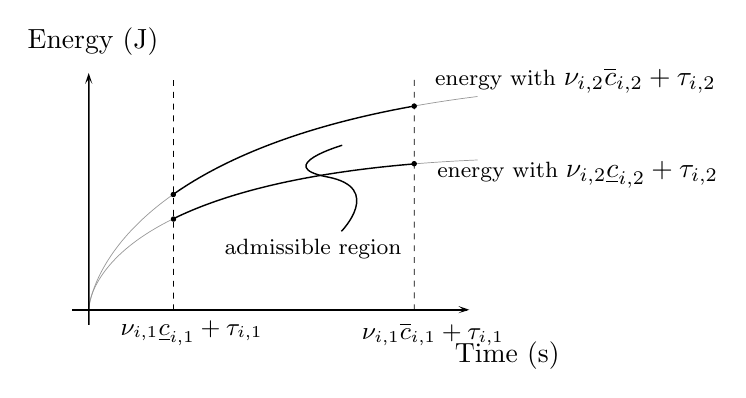
\begin{tikzpicture}[y=0.80pt, x=0.80pt, yscale=-\globalscale, xscale=\globalscale, inner sep=0pt, outer sep=0pt]
\path[fill=black,line join=round,line width=0.256pt] (62.6830,117.8310) -- (62.6830,115.1650) -- (63.0030,115.1650) -- (63.0030,117.8310) -- (62.6830,117.8310) -- cycle(62.6830,112.4980) -- (62.6830,109.8310) -- (63.0030,109.8310) -- (63.0030,112.4980) -- (62.6830,112.4980) -- cycle(62.6830,107.1650) -- (62.6830,104.4980) -- (63.0030,104.4980) -- (63.0030,107.1650) -- (62.6830,107.1650) -- cycle(62.6830,101.8310) -- (62.6830,99.1647) -- (63.0030,99.1647) -- (63.0030,101.8310) -- (62.6830,101.8310) -- cycle(62.6830,96.4980) -- (62.6830,93.8313) -- (63.0030,93.8313) -- (63.0030,96.4980) -- (62.6830,96.4980) -- cycle(62.6830,91.1647) -- (62.6830,88.4980) -- (63.0030,88.4980) -- (63.0030,91.1647) -- (62.6830,91.1647) -- cycle(62.6830,85.8313) -- (62.6830,83.1647) -- (63.0030,83.1647) -- (63.0030,85.8313) -- (62.6830,85.8313) -- cycle(62.6830,80.4980) -- (62.6830,77.8313) -- (63.0030,77.8313) -- (63.0030,80.4980) -- (62.6830,80.4980) -- cycle(62.6830,75.1647) -- (62.6830,72.4980) -- (63.0030,72.4980) -- (63.0030,75.1647) -- (62.6830,75.1647) -- cycle(62.6830,69.8313) -- (62.6830,67.1647) -- (63.0030,67.1647) -- (63.0030,69.8313) -- (62.6830,69.8313) -- cycle(62.6830,64.4980) -- (62.6830,61.8313) -- (63.0030,61.8313) -- (63.0030,64.4980) -- (62.6830,64.4980) -- cycle(62.6830,59.1647) -- (62.6830,56.4980) -- (63.0030,56.4980) -- (63.0030,59.1647) -- (62.6830,59.1647) -- cycle(62.6830,53.8313) -- (62.6830,51.1647) -- (63.0030,51.1647) -- (63.0030,53.8313) -- (62.6830,53.8313) -- cycle(62.6830,48.4980) -- (62.6830,45.8313) -- (63.0030,45.8313) -- (63.0030,48.4980) -- (62.6830,48.4980) -- cycle(62.6830,43.1647) -- (62.6830,40.4980) -- (63.0030,40.4980) -- (63.0030,43.1647) -- (62.6830,43.1647) -- cycle(62.6830,37.8313) -- (62.6830,35.1647) -- (63.0030,35.1647) -- (63.0030,37.8313) -- (62.6830,37.8313) -- cycle(62.6830,32.4980) -- (62.6830,29.8313) -- (63.0030,29.8313) -- (63.0030,32.4980) -- (62.6830,32.4980) -- cycle(62.6830,27.1647) -- (62.6830,24.4980) -- (63.0030,24.4980) -- (63.0030,27.1647) -- (62.6830,27.1647) -- cycle(62.6830,21.8313) -- (62.6830,19.1647) -- (63.0030,19.1647) -- (63.0030,21.8313) -- (62.6830,21.8313) -- cycle(62.6830,123.1650) -- (62.6830,120.4980) -- (63.0030,120.4980) -- (63.0030,123.1650) -- (62.6830,123.1650) -- cycle;



\path[fill=black,line join=round,line width=0.160pt] (22.9450,20.9131) -- (24.6859,18.4954) -- (26.1983,20.9021) -- (24.5623,15.9462) -- (22.9450,20.9131) -- cycle;



\path[fill=black,line join=round,line width=0.160pt] (191.5620,121.2300) -- (193.9450,123.0010) -- (191.5070,124.4830) -- (196.4950,122.9340) -- (191.5620,121.2300) -- cycle;



\path[cm={{1.0,0.0,0.0,1.0,(190.0,150.0)}}] (0.0000,0.0000) node[above right] () {Time (s)};



\path[cm={{1.0,0.0,0.0,1.0,(-3.0,8.0)}}] (0.0000,0.0000) node[above right] () {Energy (J)};



\path[cm={{1.0,0.0,0.0,1.0,(39.0,139.0)}}] (0.0000,0.0000) node[above right] () {\small $\nu_{i,1}\underline{c}_{i,1}+\tau_{i,1}$};



\path[cm={{1.0,0.0,0.0,1.0,(148.0,139.0)}}] (0.0000,0.0000) node[above right] () {\small $\nu_{i,1}\overline{c}_{i,1}+\tau_{i,1}$};



\path[draw=c989898,line join=round,line width=0.256pt] (24.5518,122.8240) .. controls (24.5518,122.8240) and (26.0544,96.6194) .. (62.7587,70.7926);



\path[draw=black,line join=round,line width=0.512pt] (62.7587,70.7926) .. controls (84.4429,55.5347) and (118.4130,40.4084) .. (171.6190,30.8952);



\path[draw=c989898,line join=round,line width=0.256pt] (171.6190,30.8952) .. controls (180.5780,29.2933) and (190.0820,27.8506) .. (200.1650,26.5931);



\path[draw=black,fill=black,line join=round,line width=0.512pt] (62.7778,69.9825) .. controls (63.2741,69.9825) and (63.6765,70.3848) .. (63.6765,70.8811) .. controls (63.6765,71.3774) and (63.2741,71.7798) .. (62.7778,71.7798) .. controls (62.2815,71.7798) and (61.8791,71.3774) .. (61.8791,70.8811) .. controls (61.8791,70.3848) and (62.2815,69.9825) .. (62.7778,69.9825) -- cycle;



\path[draw=black,fill=black,line join=round,line width=0.512pt] (171.5790,30.0319) .. controls (172.0750,30.0319) and (172.4780,30.4342) .. (172.4780,30.9306) .. controls (172.4780,31.4269) and (172.0750,31.8292) .. (171.5790,31.8292) .. controls (171.0830,31.8292) and (170.6800,31.4269) .. (170.6800,30.9306) .. controls (170.6800,30.4342) and (171.0830,30.0319) .. (171.5790,30.0319) -- cycle;



\path[fill=black,line join=round,line width=0.256pt] (171.4440,117.7800) -- (171.4440,115.1130) -- (171.7640,115.1130) -- (171.7640,117.7800) -- (171.4440,117.7800) -- cycle(171.4440,112.4470) -- (171.4440,109.7800) -- (171.7640,109.7800) -- (171.7640,112.4470) -- (171.4440,112.4470) -- cycle(171.4440,107.1130) -- (171.4440,104.4470) -- (171.7640,104.4470) -- (171.7640,107.1130) -- (171.4440,107.1130) -- cycle(171.4440,101.7800) -- (171.4440,99.1133) -- (171.7640,99.1133) -- (171.7640,101.7800) -- (171.4440,101.7800) -- cycle(171.4440,96.4466) -- (171.4440,93.7800) -- (171.7640,93.7800) -- (171.7640,96.4466) -- (171.4440,96.4466) -- cycle(171.4440,91.1133) -- (171.4440,88.4466) -- (171.7640,88.4466) -- (171.7640,91.1133) -- (171.4440,91.1133) -- cycle(171.4440,85.7800) -- (171.4440,83.1133) -- (171.7640,83.1133) -- (171.7640,85.7800) -- (171.4440,85.7800) -- cycle(171.4440,80.4466) -- (171.4440,77.7800) -- (171.7640,77.7800) -- (171.7640,80.4466) -- (171.4440,80.4466) -- cycle(171.4440,75.1133) -- (171.4440,72.4466) -- (171.7640,72.4466) -- (171.7640,75.1133) -- (171.4440,75.1133) -- cycle(171.4440,69.7800) -- (171.4440,67.1133) -- (171.7640,67.1133) -- (171.7640,69.7800) -- (171.4440,69.7800) -- cycle(171.4440,64.4466) -- (171.4440,61.7800) -- (171.7640,61.7800) -- (171.7640,64.4466) -- (171.4440,64.4466) -- cycle(171.4440,59.1133) -- (171.4440,56.4466) -- (171.7640,56.4466) -- (171.7640,59.1133) -- (171.4440,59.1133) -- cycle(171.4440,53.7800) -- (171.4440,51.1133) -- (171.7640,51.1133) -- (171.7640,53.7800) -- (171.4440,53.7800) -- cycle(171.4440,48.4466) -- (171.4440,45.7800) -- (171.7640,45.7800) -- (171.7640,48.4466) -- (171.4440,48.4466) -- cycle(171.4440,43.1133) -- (171.4440,40.4466) -- (171.7640,40.4466) -- (171.7640,43.1133) -- (171.4440,43.1133) -- cycle(171.4440,37.7800) -- (171.4440,35.1133) -- (171.7640,35.1133) -- (171.7640,37.7800) -- (171.4440,37.7800) -- cycle(171.4440,32.4466) -- (171.4440,29.7800) -- (171.7640,29.7800) -- (171.7640,32.4466) -- (171.4440,32.4466) -- cycle(171.4440,27.1133) -- (171.4440,24.4466) -- (171.7640,24.4466) -- (171.7640,27.1133) -- (171.4440,27.1133) -- cycle(171.4440,21.7800) -- (171.4440,19.1133) -- (171.7640,19.1133) -- (171.7640,21.7800) -- (171.4440,21.7800) -- cycle(171.4440,123.1130) -- (171.4440,120.4470) -- (171.7640,120.4470) -- (171.7640,123.1130) -- (171.4440,123.1130) -- cycle;



\path[draw=c989898,line join=round,line width=0.256pt] (24.5520,123.0820) .. controls (24.5520,123.0820) and (23.8433,100.8920) .. (62.8813,81.7576);



\path[draw=black,line join=round,line width=0.512pt] (17.2231,122.9490) -- (195.3340,122.9490);



\path[draw=black,line join=round,line width=0.512pt] (62.8813,81.7576) .. controls (84.5833,71.1203) and (118.5690,61.4270) .. (171.7890,57.0149);



\path[draw=c989898,line join=round,line width=0.256pt] (171.7890,57.0149) .. controls (180.7280,56.2738) and (190.2100,55.6817) .. (200.2670,55.2591);



\path[line join=round,line width=0.160pt] (63.4905,81.6091) -- (63.1530,83.6113);



\path[draw=black,fill=black,line join=round,line width=0.512pt] (62.8605,81.0530) .. controls (63.3568,81.0530) and (63.7592,81.4554) .. (63.7592,81.9517) .. controls (63.7592,82.4480) and (63.3568,82.8503) .. (62.8605,82.8503) .. controls (62.3642,82.8503) and (61.9619,82.4480) .. (61.9619,81.9517) .. controls (61.9619,81.4554) and (62.3642,81.0530) .. (62.8605,81.0530) -- cycle;



\path[draw=black,fill=black,line join=round,line width=0.512pt] (171.5870,56.0401) .. controls (172.0840,56.0401) and (172.4860,56.4425) .. (172.4860,56.9388) .. controls (172.4860,57.4352) and (172.0840,57.8375) .. (171.5870,57.8375) .. controls (171.0910,57.8375) and (170.6890,57.4352) .. (170.6890,56.9388) .. controls (170.6890,56.4425) and (171.0910,56.0401) .. (171.5870,56.0401) -- cycle;



\path[draw=black,line join=round,line width=0.512pt] (139.0820,48.6017) .. controls (139.0820,48.6017) and (107.0790,58.0876) .. (132.4830,62.9469) .. controls (157.8860,67.8063) and (138.7220,87.4760) .. (138.7220,87.4760);



\path[cm={{1.0,0.0,0.0,1.0,(86.0,100.0)}}] (0.0000,0.0000) node[above right] () {\footnotesize admissible region};



\path[cm={{1.0,0.0,0.0,1.0,(181.0,25.0)}}] (0.0000,0.0000) node[above right] () {\footnotesize energy with {\normalsize $\nu_{i,2}\overline{c}_{i,2}+\tau_{i,2}$}};



\path[cm={{1.0,0.0,0.0,1.0,(182.0,68.0)}}] (0.0000,0.0000) node[above right] () {\footnotesize energy with {\normalsize $\nu_{i,2}\underline{c}_{i,2}+\tau_{i,2}$}};



\path[draw=black,line join=round,line width=0.512pt] (24.6557,129.7240) -- (24.6562,17.3508);




\end{tikzpicture}

  \caption[Concept of a path and computations parameters scale transformation]{The concept of a path and computations parameters scale transformation. Without any battery constraints, the energy-aware coverage planning and scheduling select the highest configuration which respects the control constraint (admissible region) from \frefeq{eq:constraint-set}.}
  \label{fig:plot-6}
  \efr
\end{figure}

The scaling factors for the computations parameters from \frefeq{eq:scaling} are derived using {\small\tt{powprofiler}}, the open-source modeling tool from \fref{sec:powprof}{Section}. We estimate the energy cost of a given schedule (a given computations configuration) with the function $g$ from \fref{def:comp-ener}{Definition}. 
For instance, if the computation is the CNN ROS node, the computation parameter $c_{1,2}$ corresponds to the \Gls{acr:fps} rate. The tool then measures power according to the detection frequency.

The scaling factors add the computational energy component to the model in \frefeq{eq:state-perf}. They are derived similarly to \frefeq{eq:scale-traj}
\begin{subequations}\label{eq:scale-comp}\begin{align}
  \nu_{i,j}&=(g(\overline{c}_{i,j})-g(\underline{c}_{i,j}))/(\overline{c}_{i,j}-\underline{c}_{i,j}),\\
  \tau_{i,j}&=\underline{c}_{i,j}(g(\underline{c}_{i,j})-g(\overline{c}_{i,j}))/(\overline{c}_{i,j}-\underline{c}_{i,j})+g(\underline{c}_{i,j}),
\end{align}\end{subequations}
$\forall j\in[\rho+1,n]$. We then assume $g$ only returns the power metric (so we do not specify an additional parameter to numerate the metric) and, for ease of notation, assume all the values from $g(\underline{c}_{i,j})$ to $g(\underline{c}_{i,j})$ are distributed linearly. Moreover, let the factors be zero when the parameters $c_i^\sigma=\emptyset$.

The concept of a path and a computation parameter $(c_{i,1},c_{i,2})$ scale transformation is illustrated in \fref{fig:plot-6}{Figure}. 
The energy domain is bounded by the output of the \powprof{} tool, while the flight time domain is by the empirical data. The energy-aware coverage planning and scheduling select the highest possible configuration of parameters (control) in the admissible region\findex{admissible region} (under the constraints). 
\begin{figure}[h!]
  \sfr
  \centering
  \fontfamily{phv}\selectfont
  
\definecolor{cECECEC}{RGB}{236,236,236}
\definecolor{cFFFFFF}{RGB}{255,255,255}

\def \globalscale {1.000000}
\begin{tikzpicture}[y=0.80pt, x=0.80pt, yscale=-\globalscale, xscale=\globalscale, inner sep=0pt, outer sep=0pt]
\path[fill=cECECEC,line join=round,line width=0.512pt,rounded corners=0.0000cm] (87.8254,28.6703) rectangle (287.0154,141.7963);



\path[draw=black,line join=round,line width=0.512pt] (81.2745,114.4430) -- (220.9180,22.5329);



\path[draw=black,line join=round,line width=0.512pt] (81.2745,110.4430) -- (214.8400,22.5329);



\path[draw=black,line join=round,line width=0.512pt] (81.2745,106.4430) -- (208.7630,22.5329);



\path[draw=black,line join=round,line width=0.512pt] (81.2745,102.4430) -- (202.6850,22.5329);



\path[draw=black,line join=round,line width=0.512pt] (81.2745,126.4430) -- (239.1500,22.5329);



\path[draw=black,line join=round,line width=0.512pt] (81.2745,130.4430) -- (245.2270,22.5329);



\path[draw=black,line join=round,line width=0.512pt] (81.2745,134.4430) -- (251.3050,22.5329);



\path[draw=black,line join=round,line width=0.512pt] (81.2745,138.4430) -- (257.3820,22.5329);



\path[draw=black,line join=round,line width=0.512pt] (81.2745,98.4426) -- (196.6080,22.5329);



\path[draw=black,line join=round,line width=0.512pt] (81.2745,94.4426) -- (190.5310,22.5329);



\path[draw=black,line join=round,line width=0.512pt] (81.2745,90.4426) -- (184.4530,22.5329);



\path[draw=black,line join=round,line width=0.512pt] (81.2745,86.4426) -- (178.3760,22.5329);



\path[draw=black,line join=round,line width=0.512pt] (81.2745,118.4430) -- (226.9950,22.5329);



\path[draw=black,line join=round,line width=0.512pt] (81.2745,122.4430) -- (233.0720,22.5329);



\path[draw=black,line join=round,line width=0.512pt] (81.2745,54.9620) -- (130.5460,22.5329);



\path[draw=black,line join=round,line width=0.512pt] (81.2745,50.9620) -- (124.4680,22.5329);



\path[draw=black,line join=round,line width=0.512pt] (81.2745,46.9620) -- (118.3910,22.5329);



\path[draw=black,line join=round,line width=0.512pt] (81.2745,42.9620) -- (112.3130,22.5329);



\path[draw=black,line join=round,line width=0.512pt] (81.2745,66.9620) -- (148.7780,22.5329);



\path[draw=black,line join=round,line width=0.512pt] (81.2745,70.9620) -- (154.8550,22.5329);



\path[draw=black,line join=round,line width=0.512pt] (81.2745,74.9620) -- (160.9330,22.5329);



\path[draw=black,line join=round,line width=0.512pt] (81.2745,78.9620) -- (167.0100,22.5329);



\path[draw=black,line join=round,line width=0.512pt] (81.2745,82.4426) -- (172.2980,22.5329);



\path[draw=black,line join=round,line width=0.512pt] (81.2745,38.9620) -- (106.2360,22.5329);



\path[draw=black,line join=round,line width=0.512pt] (81.2745,34.9620) -- (100.1590,22.5329);



\path[draw=black,line join=round,line width=0.512pt] (136.6230,22.5329) -- (81.2745,58.9620);



\path[draw=black,line join=round,line width=0.512pt] (81.2745,62.9620) -- (142.7000,22.5329);



\path[draw=black,line join=round,line width=0.512pt] (123.0100,147.4920) -- (292.9440,35.6462);



\path[draw=black,line join=round,line width=0.512pt] (116.9330,147.4920) -- (292.9440,31.6462);



\path[draw=black,line join=round,line width=0.512pt] (110.8560,147.4920) -- (292.9440,27.6462);



\path[draw=black,line join=round,line width=0.512pt] (141.2430,147.4920) -- (292.9440,47.6462);



\path[draw=black,line join=round,line width=0.512pt] (147.3200,147.4920) -- (292.9440,51.6462);



\path[draw=black,line join=round,line width=0.512pt] (153.3970,147.4920) -- (292.9440,55.6462);



\path[draw=black,line join=round,line width=0.512pt] (159.4750,147.4920) -- (292.9440,59.6462);



\path[draw=black,line join=round,line width=0.512pt] (98.7008,147.4920) -- (288.5580,22.5329);



\path[draw=black,line join=round,line width=0.512pt] (92.6234,147.4920) -- (282.4810,22.5329);



\path[draw=black,line join=round,line width=0.512pt] (81.2745,142.9620) -- (264.2490,22.5329);



\path[draw=black,line join=round,line width=0.512pt] (81.2745,146.9620) -- (270.3260,22.5329);



\path[draw=black,line join=round,line width=0.512pt] (129.0880,147.4920) -- (292.9440,39.6462);



\path[draw=black,line join=round,line width=0.512pt] (135.1650,147.4920) -- (292.9440,43.6462);



\path[draw=black,line join=round,line width=0.512pt] (274.9460,147.4920) -- (292.9440,135.6460);



\path[draw=black,line join=round,line width=0.512pt] (268.8680,147.4920) -- (292.9440,131.6460);



\path[draw=black,line join=round,line width=0.512pt] (262.7910,147.4920) -- (292.9440,127.6460);



\path[draw=black,line join=round,line width=0.512pt] (214.1710,147.4920) -- (292.9440,95.6462);



\path[draw=black,line join=round,line width=0.512pt] (208.0940,147.4920) -- (292.9440,91.6462);



\path[draw=black,line join=round,line width=0.512pt] (202.0170,147.4920) -- (292.9440,87.6462);



\path[draw=black,line join=round,line width=0.512pt] (195.9390,147.4920) -- (292.9440,83.6462);



\path[draw=black,line join=round,line width=0.512pt] (232.4040,147.4920) -- (292.9440,107.6460);



\path[draw=black,line join=round,line width=0.512pt] (238.4810,147.4920) -- (292.9440,111.6460);



\path[draw=black,line join=round,line width=0.512pt] (244.5590,147.4920) -- (292.9440,115.6460);



\path[draw=black,line join=round,line width=0.512pt] (250.6360,147.4920) -- (292.9440,119.6460);



\path[draw=black,line join=round,line width=0.512pt] (256.7130,147.4920) -- (292.9440,123.6460);



\path[draw=black,line join=round,line width=0.512pt] (189.8620,147.4920) -- (292.9440,79.6462);



\path[draw=black,line join=round,line width=0.512pt] (183.7840,147.4920) -- (292.9440,75.6462);



\path[draw=black,line join=round,line width=0.512pt] (177.7070,147.4920) -- (292.9440,71.6462);



\path[draw=black,line join=round,line width=0.512pt] (165.5520,147.4920) -- (292.9440,63.6462);



\path[draw=black,line join=round,line width=0.512pt] (171.6300,147.4920) -- (292.9440,67.6462);



\path[draw=black,line join=round,line width=0.512pt] (220.2490,147.4920) -- (292.9440,99.6462);



\path[draw=black,line join=round,line width=0.512pt] (226.3260,147.4920) -- (292.9440,103.6460);



\path[draw=black,line join=round,line width=0.512pt] (86.5460,147.4920) -- (276.4030,22.5329);



\path[draw=black,line join=round,line width=0.512pt] (104.7780,147.4920) -- (292.9440,23.6462);



\path[fill=cFFFFFF,line join=round,even odd rule,line width=0.512pt] (96.8091,15.9084) -- (296.1540,19.5982) -- (294.8280,139.1820) -- (246.6580,53.9253) -- (94.4984,22.9653) -- (96.8091,15.9084) -- cycle;



\path[draw=black,fill=cFFFFFF,line join=round,line width=0.512pt] (87.8254,28.6703) -- (240.4110,59.6693) -- (287.0160,141.7960) -- (87.8254,141.7960) -- (87.8254,28.6703) -- cycle;



\path[fill=black,line join=round,line width=0.160pt] (40.2846,16.3558) -- (42.5576,14.3509) -- (44.6410,16.3467) -- (42.4551,10.5783) -- (40.2846,16.3558) -- cycle;



\path[fill=black,line join=round,line width=0.160pt] (311.2300,168.8650) -- (313.2060,171.1630) -- (311.1840,173.2210) -- (316.9790,171.1080) -- (311.2300,168.8650) -- cycle;



\path[draw=black,line join=round,line width=0.512pt] (33.7496,171.1390) -- (314.8740,171.1390);



\path[draw=black,line join=round,line width=0.512pt] (42.5583,179.1700) -- (42.5588,12.9691);


\path[cm={{1.0,0.0,0.0,1.0,(324.0,194.0)}}] (0.0000,0.0000) node[above right] () {\footnotesize flight time};



\path[cm={{1.0,0.0,0.0,1.0,(0.0,6.0)}}] (0.0000,0.0000) node[above right] () {\footnotesize energy};



\path[cm={{1.0,0.0,0.0,1.0,(58.0,159)}}] (0.0000,0.0000) node[above right] () {$\neg\mathcal{U}_i$};





\path[cm={{1.0,0.0,0.0,1.0,(114.0,119.0)}}] (0.0000,0.0000) node[above right] () {$\mathcal{U}_i\wedge \mathcal{Y}$};



\path[fill=cECECEC,line join=round,even odd rule,line width=0.512pt] (271.4110,28.5172) -- (286.8770,28.5703) -- (287.0190,125.3610) -- (246.6320,53.8773) -- (122.6190,28.6772) -- (271.4110,28.5172) -- cycle;



\path[fill=foo,line join=round,line width=0.160pt] (240.4120,58.7857) .. controls (240.9260,58.7857) and (241.3420,59.2021) .. (241.3420,59.7157) .. controls (241.3420,60.2293) and (240.9260,60.6457) .. (240.4120,60.6457) .. controls (239.8990,60.6457) and (239.4820,60.2293) .. (239.4820,59.7157) .. controls (239.4820,59.2021) and (239.8990,58.7857) .. (240.4120,58.7857) -- cycle;



\path[cm={{1.0,0.0,0.0,1.0,(258.0,57.0)}}] (0.0000,0.0000) node[above right] () {$\neg\mathcal{Y}$};



\path[cm={{1.0,0.0,0.0,1.0,(225.0,79.0)}}] (0.0000,0.0000) node[above right] () {\color{foo}$c_i^*$};




\end{tikzpicture}


  \caption[Change in the admissible region]{Change in the admissible region in \fref{fig:plot-6}{Figure} due to a battery constraint.}
  \label{fig:plot-7}
  \efr
\end{figure}
Currently, the highest control corresponds to $(\overline{c}_{i,1},\overline{c}_{i,2})$. We will see in \fref{sec:output-mpc}{Section} the optimal control derivation over a time horizon $N$ under given battery constraints.
In \fref{fig:plot-7}{Figure} we briefly exemplify this latter case, where due to, e.g., a sudden battery drop, the energy and time domains are shrunk. The highest possible control is thus now different from the above scenario.

\subsection{\color{red}Aperiodic energy evolution}
\label{sec:non-perio}


%%%%%%%%%%%%%%%%%
\section{\color{red}Summary}

